\documentclass[17pt]{extarticle}
\usepackage{../mystyle}
\begin{document}

\section{Задача принятия решений. Типы задач принятия решений}

Есть некая среда. В этой среде есть управляющая и управляемая подсистемы.
Управляющая подсистема посылает управляющие воздействия(УВ) \\ управляемой подсистеме.

\begin{enumerate}
    \item Управляющая подсистема может воздействовать на объект управления с помощью альтернативных управляющих воздействий: УВ1, УВ2, УВn
    \item Состояние Объекта управления определяется двумя факторами: \\ выбранным УВ; состоянием среды
    \item Принципиальным является следующее обстоятельство:
          Управляющая подсистема не может воздействовать на среду, более того, она, как правило, не имеет полной информации о состоянии среды
    \item Цель Управляющей подсистемы: перевести объект управления в наиболее предпочтительное для себя состояние,
          используя для этого любое УВ, имеющееся в ее распоряжении
    \item Выбор Управляющей подсистемой конкретного УВ (допустимой альтернативы, допустимого решения)
          называется \textbf{принятием решения}.
\end{enumerate}

При принятии решения основной задачей является нахождение оптимального решения.
На содержательном уровне оптимальное решение можно определить как наилучшее в следующем смысле:
оптимальное решение в наибольшей степени соответствует цели
Управляющей подсистемы в рамках имеющейся у нее информации о состоянии среды.

В зависимости от информации,
которую имеет при принятии решения \\ управляющая подсистема относительно состояния среды,
различают несколько основных типов задач принятия решения.

\begin{enumerate}
    \item \textit{Принятие решения в условиях определенности} характеризуется тем, \\
          что состояние среды является фиксированным (неизменным), причем управляющая система «знает», в каком состоянии находится среда.

    \item \textit{Принятие решения в условиях риска} означает,
          что управляющая подсистема имеет информацию стохастического характера о поведении среды
          (например, ей известно распределение вероятностей на множестве состояний среды).

    \item \textit{Принятие решения происходит в условиях неопределенности},
          если никакой дополнительной информации (кроме знания самого множества возможных состояний среды) управляющая подсистема не имеет.

    \item \textit{Принятие решения в теоретико-игровых условиях} имеет место тогда,
          когда среду можно трактовать как одну или несколько целенаправленных управляющих подсистем.
          В этом случае математическая модель принятия решения называется \textbf{теоретико-игровой моделью} (игрой).
\end{enumerate}



\section{Линейное программирование. Постановка \\ задачи планирования производства, составление смеси (о диете).}
\subsection{Линейное программирование}

\begin{definition}
    Задача, состоящая в нахождении наибольшего (наименьшего) значения целевой функции
    \(
    f = C_1 X_1 + C_2 X_2 + \cdots + C_n X_n \xrightarrow{?} \max(\min)
    \)
    на множестве точек \( x = (x_1, \ldots, x_n) \), удовлетворяющих системе ограничений вида
    \[
        \begin{cases}
            a_{11}x_1 + a_{12}x_2 + \cdots + a_{1n}x_n \, R_1 \, b_1 \\
            a_{21}x_1 + a_{22}x_2 + \cdots + a_{2n}x_n \, R_2 \, b_2 \\
            \vdots                                                   \\
            a_{m1}x_1 + a_{m2}x_2 + \cdots + a_{mn}x_n \, R_n \, b_m
        \end{cases}
    \]
    называется \textbf{задачей линейного программирования общего вида}.
    Здесь:
    \begin{itemize}
        \item \( R_i, i = \overline{1, m} \) — один из знаков \( =, \geq, \leq \);
        \item \( C_j, j = \overline{1, n} \) и \( a_{ij}, i = \overline{1, m}, j = \overline{1, n} \) — заданные константы.
    \end{itemize}
\end{definition}

\begin{definition}
    Всякую точку \( X = (x_1, \ldots, x_n) \), компоненты которой удовлетворяют системе ограничений,
    будем называть допустимой точкой или допустимым решением задачи, или допустимым планом задачи.
\end{definition}

Задача линейного программирования состоит в нахождении такой допустимой точки \( x \) (такого допустимого плана) среди множества допустимых точек,
при которой целевая функция принимает \textbf{max(min)} значение.

\begin{definition}
    Допустимое решение \( x^{(0)} = (x_1^{(0)}, \ldots, x_n^{(0)}) \),
    доставляющее целевой функции оптимальное значение (оптимум),
    будем называть оптимальным решением или оптимальным планом задачи.
\end{definition}

\begin{definition}
    Задача об оптимальном плане производства продукции
    \begin{itemize}
        \item $n$ видов продукции, $j = 1, n;$
        \item $m$ видов ресурсов (сырья), $i = 1, m;$
        \item $a_{ij}$ - количество ресурса вида $i$, требующегося для производства единицы продукции вида $j$
        \item $b_i$ - запасы ресурса вида $i$, $\quad i = 1, m$
        \item $c_j$ - доход (прибыль) от реализации единицы продукции вида $j$
    \end{itemize}
    Необходимо найти такой план производства продукции, при котором \\ достигается максимальная прибыль,
    для реализации которого достаточно имеющихся ресурсов.

    \[
        f = c_1 x_1 + \ldots + c_n x_n \rightarrow \max
    \]

    \[
        \begin{cases}
            a_{11} x_1 + \ldots + a_{1n} x_n \leq b_1 \\
            \ldots                                    \\
            a_{m1} x_1 + \ldots + a_{mn} x_n \leq b_m
        \end{cases} x_j \geq 0, \quad j = \overline{1, n}
    \]
\end{definition}


\begin{definition}[Задача о диете (исторически одна из самых первых)]
    Условия:
    \begin{itemize}
        \item \( n \) — видов кормов, \( j =\overline{1, n} \);
        \item \( m \) — видов питательных веществ, \( i =\overline{1, m} \);
        \item \( a_{ij} \) — содержание \( i \)-го вида питательного вещества в единице \( j \)-го вида корма;
        \item \( b_i \) — необходимый минимум \( i \)-го питательного вещества в день, \( i=\overline{1,m} \);
        \item \( c_j \) — стоимость единицы \( j \)-го вида корма.
    \end{itemize}

    Необходимо составить рацион, имеющий минимальную стоимость, в котором содержание каждого вида питательных веществ было бы не менее установленного предела.

    \[
        f = c_1 x_1 + \cdots + c_n x_n \rightarrow \min
    \]

    \[
        \begin{cases}
            a_{11} x_1 + \cdots + a_{1n} x_n \geq b_1 \\
            \vdots                                    \\
            a_{m1} x_1 + \cdots + a_{mn} x_n \geq b_m
        \end{cases} x_j \geq 0, \quad j = 1, n
    \]
\end{definition}




\section{Постановка задачи линейного программирования в общей форме}
хз, смотри предыдущий вопрос. В лекциях именно общей формы нет.


\section{Геометрическая интерпретация двумерной задачи линейного программирования}

Рассмотрим двумерную задачу: \(F = c_1 x_1 + c_2 x_2 \rightarrow \max\)

\[
    \begin{cases}
        a_{11}x_1 + a_{12}x_2 \leq b_1 \\
        a_{21}x_1 + a_{22}x_2 \leq b_2 \\
        \vdots                         \\
        a_{m1}x_1 + a_{m2}x_2 \leq b_m
    \end{cases}
\]

Каждое из ограничений \( a_{i1} x_1 + a_{i2} x_2 \leq b_i \) определяет в плоскости с системой координат \( x_1, 0, x_2 \) множество точек,
лежащих по одну сторону от прямой \( a_{i1} x_1 + a_{i2} x_2 = b_i \) (т.е. полуплоскость).

Множество всех точек плоскости, координаты которых удовлетворяют \\ всем ограничениям, т.е. принадлежат сразу всем полуплоскостям,
определяемым отдельными ограничениями, будет представлять собой допустимое множество.

Пусть допустимая область задачи оказалась непустой. \\
Мы хотим найти те точки допустимой области, координаты которых дают
целевой функции наибольшее значение.
Построим линию уровня целевой функции $F = c_1 x_1 + c_2 x_2 = \alpha$.
Перемещая линию уровня в направлении вектора $grad(G)=(c_1, c_2)=\overline{n}$,
нормального к линии уровня, будем получать в пересечении этой линии
с допустимой областью точки, в которых целевая функция принимает
новое значение, большее, чем на предшествующих линиях уровня.
Пересечение допустимой области с линией уровня в том ее положении,
когда дальнейшее перемещение дает пустое множество, и будет
множеством оптимальных точек задачи линейного программирования.

Случаи при решении ЗЛП:
\begin{itemize}
    \item Решение достигается в угловой точке
    \item Целевая функция не ограничена
    \item Бесконечное множество решений
\end{itemize}


\section{Свойства задачи линейного \\ программирования}

\begin{definition}
    Множество \( D \) — точек \( n \)-мерного евклидова пространства будем называть выпуклым, если
    \[
        \forall x^{(1)} = (x_1^{(1)}, \ldots, x_n^{(1)}), x^{(2)} = (x_1^{(2)}, \ldots, x_n^{(2)})
        \quad \forall \alpha \geq 0, \beta \geq 0 \colon \alpha + \beta = 1
    \]
    точка \(x = \alpha x^{(1)} + \beta x^{(2)}\) также принадлежит \( D \).
\end{definition}

\begin{definition}
    Вершиной выпуклого множества в \( \mathbb{R}^n \) назовём такую точку, которую нельзя представить в виде
    \(
    x = \alpha x^{(1)} + \beta x^{(2)}, \quad \alpha > 0, \beta > 0 \colon \alpha + \beta = 1
    \)
    ни при каких \(x^{(1)}, x^{(2)}\).
\end{definition}

\subsection{Свойства ЗЛП}
\begin{enumerate}
    \item Допустимая область ЗЛП выпукла, если она не пуста.
    \item Если допустимая область имеет вершины и ЗЛП имеет решение, то оно достигается по крайней мере в одной из вершин.
    \item Множество решений ЗЛП выпукло.
    \item Если допустимая область ограничена, то ЗЛП имеет оптимальное решение.
    \item Необходимым и достаточным условием существования решения ЗЛП на максимум(минимум) является
          ограниченность целевой функции сверху(соответственно снизу) в допустимой области.
\end{enumerate}



\section{Приведение задачи линейного программирования к каноническому виду. Формы записи задач ЛП.}
\begin{definition}
    Задачу ЗЛП, представленную в виде
    \(
    f = C_1 X_1 + C_2 X_2 + \cdots + C_n X_n \xrightarrow{?} \max(\min), x = (x_1, \ldots, x_n) \colon x_i \geq 0, i=\overline{1,n} \)
    \[
        \begin{cases}
            a_{11}x_1 + a_{12}x_2 + \cdots + a_{1n}x_n = b_1 \\
            a_{21}x_1 + a_{22}x_2 + \cdots + a_{2n}x_n = b_2 \\
            \vdots                                           \\
            a_{m1}x_1 + a_{m2}x_2 + \cdots + a_{mn}x_n = b_m
        \end{cases}
    \]
    называется \textbf{канонической ЗЛП}.
\end{definition}

\begin{algorithm}
    \caption{Приведение ЗЛП к каноническому виду}
    \begin{algorithmic}[1]
        \If{\( f \to \max \)}
        \State Заменить \( f \) на \( -f \) и минимизировать: \( f \to \min \).
        \EndIf

        \For{каждого ограничения \( i = 1, 2, \dots, m \)}
        \If{\( R_i = \leq \)}
        \State Добавить неотрицательную дополнительную переменную \( s_i \geq 0 \):
        \[
            a_{i1}x_1 + a_{i2}x_2 + \cdots + a_{in}x_n + s_i = b_i.
        \]
        \ElsIf{\( R_i = \geq \)}
        \State Вычесть неотрицательную дополнительную переменную \( s_i \geq 0 \):
        \[
            a_{i1}x_1 + a_{i2}x_2 + \cdots + a_{in}x_n - s_i = b_i.
        \]
        \EndIf
        \EndFor

        \For{каждой переменной \( x_j, j = 1, 2, \dots, n \)}
        \If{\( x_j \) не ограничена по знаку}
        \State Заменить \( x_j \) на \( x_j^+ - x_j^- \), где \( x_j^+ \geq 0 \), \( x_j^- \geq 0 \).
        \EndIf
        \EndFor
    \end{algorithmic}
\end{algorithm}

Виды задач линейного программирования (ЛП)
\begin{enumerate}
    \item Общего вида
          \[
              \begin{cases}
                  \sum\limits_{j=1}^{n} c_j x_j \to \max                                 \\
                  \sum\limits_{j=1}^{n} a_{ij} x_j \le b_i, \quad i = \overline{1,m_1}   \\
                  \sum\limits_{j=1}^{n} a_{ij} x_j = b_i, \quad i = \overline{m_1+1,m_2} \\
                  \sum\limits_{j=1}^{n} a_{ij} x_j \ge b_i, \quad i = \overline{m_2+1,m}
              \end{cases}
          \]
    \item Неотрицательных переменных
          \[
              \begin{cases}
                  \sum\limits_{j=1}^{n} c_j x_j \to \max                               \\
                  \sum\limits_{j=1}^{n} a_{ij} x_j \le b_i, \quad i = \overline{1,m_1} \\
                  \sum\limits_{j=1}^{n} a_{ij} x_j = b_i, \quad i = \overline{m_1+1,m} \\
                  x_j \ge 0, \quad j = \overline{1,n}
              \end{cases}
          \]
    \item Стандартная форма
          \[
              \begin{cases}
                  \sum\limits_{j=1}^{n} c_j x_j \to \max                             \\
                  \sum\limits_{j=1}^{n} a_{ij} x_j \le b_i, \quad i = \overline{1,m} \\
                  x_j \ge 0, \quad j = \overline{1,n}
              \end{cases}
          \]
    \item Каноническая форма
          \[
              \begin{cases}
                  \sum\limits_{j=1}^{n} c_j x_j \to \max                           \\
                  \sum\limits_{j=1}^{n} a_{ij} x_j = b_i, \quad i = \overline{1,m} \\
                  x_j \ge 0, \quad j = \overline{1,n}
              \end{cases}
          \]
    \item Матричная стандартная форма
          \[
              \begin{cases}
                  f=(c, x) \to \max \\
                  A x \le b         \\
                  x \ge 0
              \end{cases}
          \]
\end{enumerate}


\section{Опорные точки допустимого множества. \\ Вырожденные и невырожденные опорные точки.
  Базис невырожденной опорной точки. \\ Теорема о связи опорной точки и вершины ОДР}

\[f = C_1 X_1 + C_2 X_2 + \cdots + C_n X_n \rightarrow \max, x = (x_1, \ldots, x_n) \colon x_i \geq 0, i=\overline{1,n} \]
\[
    \begin{cases}
        a_{11}x_1 + a_{12}x_2 + \cdots + a_{1n}x_n = b_1 \\
        a_{21}x_1 + a_{22}x_2 + \cdots + a_{2n}x_n = b_2 \\
        \vdots                                           \\
        a_{m1}x_1 + a_{m2}x_2 + \cdots + a_{mn}x_n = b_m
    \end{cases}
\]

Введем в рассмотрение векторы
\[
    A_j = \begin{pmatrix}
        a_{1j} \\
        a_{2j} \\
        \vdots \\
        a_{mj}
    \end{pmatrix}, j=\overline{1,n}
\]
\[
    f = (c, x) \rightarrow \max
\]
\[
    A_1 x_1 + A_2 x_2 + \dots + A_n x_n = b, x \geq 0
\]
Задачу ЛП можно трактовать следующим образом: из всех разложений вектора b по
векторам $A_1 \dots A_n$ с неотрицательными коэффициентами требуется
выбрать хотя бы одно такое, коэффициенты $x_j, j=\overline{1,n}$,
которого доставляют целевой функции f оптимальное значение.
Не ограничивая общности, считаем ранг матрицы $A$ равным $m$ и $n>m$ (случай $n=m$ тривиален).

\begin{definition}
    Ненулевое допустимое решение \( x = (x_1, \ldots, x_n) \) называется \textbf{опорным},
    если векторы \( A_j \), соответствующие отличным от нуля координатам вектора \( x \), линейно независимы.
\end{definition}

\begin{definition}
    Ненулевое опорное решение назовем \textbf{невырожденным}, если оно имеет точно \( m \) положительных координат.
\end{definition}

\begin{definition}
    Если число положительных координат опорного решения меньше \( m \), то оно называется \textbf{вырожденным}.
\end{definition}

\begin{definition}
    Упорядоченный набор из \( m \) линейно независимых векторов \( A_j \), соответствующих положительным координатам опорного решения,
    назовем \textbf{базисом}.
\end{definition}

\begin{theorem}[Теорема о связи опорного решения и вершины допустимого множества]
    Вектор \( x = (x_1, \ldots, x_n) \) тогда и только тогда является опорным решением задачи, когда точка \( x = (x_1, \ldots, x_n) \) является вершиной допустимого множества.
\end{theorem}

Таким образом, задача нахождения вершины допустимого множества свелась к задаче нахождения опорного решения, а, следовательно, к нахождению базиса.

Будем считать, что исходный базис \( A_1, A_2, \ldots, A_m \) дан.
Отправляясь от него, покажем, как найти опорное решение.
Сформулируем условие оптимальности решения, условие отсутствия решения.
Покажем, как перейти к базису, дающему лучшее решение.



\section{Основная идея симплексного метода решения задачи ЛП при известном допустимом базисном решении.}
Свойства задачи линейного программирования наталкивают на следующую схему решения задачи линейного программирования,
известную, \\
как симплекс-метод.
Пусть рассматриваемая задача имеет непустое допустимое множество с вершинами.
Тогда тем или иным способом находим какую-нибудь вершину допустимого
множества и по определенным критериям определяем, не является ли она
оптимальной.
Если она оптимальна, то задача решена. Если нет, то, используя определенные правила, проверяем,
нельзя ли утверждать, что задача не имеет оптимального решения (целевая функция не ограничена
сверху или, соответственно, снизу на допустимом множестве).
Если утверждать это можно, то задача неразрешима. Если нельзя, то по определенному правилу ищем новую,
лучшую (в смысле значения целевой функции) вершину и переходим к пункту 1.
Для реализации предложенной схемы необходимо:
\begin{itemize}
    \item указать способ нахождения вершины допустимого множества,
    \item критерии оптимальности, неразрешимости,
    \item способ перехода от одной вершины к другой, лучшей в смысле значения целевой функции.
\end{itemize}

Идея симплекс-метода состоит в том, чтобы исходя из начального опорного решения найти новое опорное
решение, исключая для этого некоторый вектор $A_s, s \in \overline{1,m}$ из начального базиса и заменяя его
одним из небазисных векторов $A_r, r \in \overline{m + 1, n}$
таким образом, чтобы новое опорное решение не ухудшало значения целевой функции.


\section{Алгоритм симплекс-метода, симплекс-таблицы}
\begin{enumerate}
    \item Для известного начального базиса находят координаты разложения векторов \( b \) и \( A_k \) \( (k = 1, \ldots, n) \) по базису:
          \[
              \begin{cases}
                  x^0 = A_B^{-1}b - \text{ненулевые координаты опорной точки}, \\
                  x^k = A_B^{-1}A_k, \, k = \overline{1,n} - \text{координаты разложения вектора } A_k \text{ по базису}.
              \end{cases}
          \]
    \item Вычисляют симплекс-разности: \(\Delta_k = c_k - c_B A_B^{-1}A_k, \, k = 1, \ldots, n. \)
    \item Проверяют план на оптимальность. Если все \(\Delta_k \leq 0\), \( k = 1, \ldots, n \), то решение оптимально.
    \item Проверяется критерий отсутствия решения.
          Если \(\exists \Delta_r > 0\): все \( x_{ir} \leq 0, i = \overline{1,m} \), то целевая функция не ограничена сверху в допустимой области.
    \item Определяют вектор \( A_r \), вводимый в базис: \(\Delta_r > 0\)
          и максимальная среди всех положительных \(\Delta_k\), \( k = \overline{1,n} \).

    \item Определяют вектор \( A_s \), выводимый из базиса:
          \[
              A_s : \frac{x_{s0}}{x_{sr}} = \min_{i \in I} \frac{x_{i0}}{x_{ir}} \quad (x_{ir} > 0) \Rightarrow \text{строим новый базис и переходим в п.1.}
          \]
\end{enumerate}
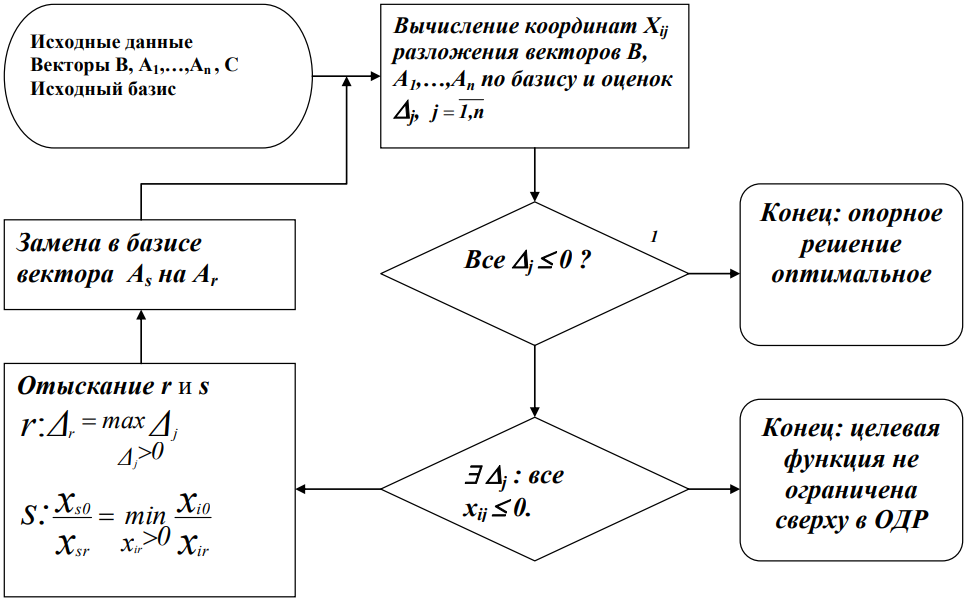
\includegraphics[width=1\textwidth]{9.png}
Формулы пересчета координат разложения векторов по новому базису:

\[
    x_{jk}' =
    \begin{cases}
        x_{jk} - \frac{x_{jr}}{x_{sr}} x_{sk}, & \text{если } j \in I \setminus s, \\
        \frac{x_{sk}}{x_{sr}},                 & \text{если } j = r.
    \end{cases}
\]

\begin{tabular}{|c|c|c|c|c|c|c|c|}
    \hline
                 &                      &                         & \( C_1 \)      & \(\cdots\) & \( C_r \)      & \(\cdots\) & \( C_n \)      \\
    \hline
    базис        & \( C_{\text{баз}} \) & \( B \)                 & \( A_1 \)      &            & \( A_r \)      &            & \( A_n \)      \\
    \hline
    \( A_{i1} \) & \( C_{i1} \)         & \( X_{10} \)            & \( X_{11} \)   &            & \( X_{1r} \)   &            & \( X_{1n} \)   \\
    \hline
    \(\vdots\)   & \(\vdots\)           & \(\vdots\)              & \(\vdots\)     &            & \(\vdots\)     &            & \(\vdots\)     \\
    \hline
    \( A_{is} \) & \( C_{is} \)         & \( X_{s0} \)            & \( X_{s1} \)   &            & \( X_{sr} \)   &            & \( X_{sn} \)   \\
    \hline
    \(\vdots\)   & \(\vdots\)           & \(\vdots\)              & \(\vdots\)     &            & \(\vdots\)     &            & \(\vdots\)     \\
    \hline
    \( A_{im} \) & \( C_{im} \)         & \( X_{m0} \)            & \( X_{mr} \)   &            & \( X_{mr} \)   &            & \( X_{mn} \)   \\
    \hline
                 &                      & \( f(x^{\text{опт}}) \) & \( \Delta_1 \) &            & \( \Delta_r \) &            & \( \Delta_n \) \\
    \hline
\end{tabular}


\section{Метод искусственного базиса поиска \\ начальной опорной точки.}
Будем считать, что для задачи
\(
\langle c, x \rangle \rightarrow \max, D: Ax = b, \, x \geq 0
\)
выполнено условие \( b \geq 0 \).

Рассмотрим вспомогательную задачу:
\[
    \sum_{i=1}^m y_i \rightarrow \max \quad (2)
\]
\[
    \tilde{D}: Ax + y = b, \, x \geq 0, \, y \geq 0
\]
\[
    \tilde{D} = \biggl\{(x, y) \in \mathbb{R}^{n+m} : \sum_{j=1}^n A_j x_j + \sum_{i=1}^m e_i y_i = b, \, x \geq 0, \, y \geq 0\biggr\}
\]
\[
    \Rightarrow
    \begin{cases}
        (\vec{0}, b) - \text{опорная точка в } D.
    \end{cases}
\]

Целевая функция вспомогательной задачи ограничена сверху нулем (0). Следовательно, эта задача имеет оптимальное решение.
\[
    G = -y_1 - y_2 - \cdots - y_m \rightarrow \max
\]
\[
    \begin{cases}
        a_{11}x_1 + \cdots + a_{1n}x_n + y_1 = b_1        \\
        a_{21}x_1 + \cdots + a_{2n}x_n + 0y_1 + y_2 = b_2 \\
        \vdots                                            \\
        a_{m1}x_1 + \cdots + a_{mn}x_n + 0y_1 + \cdots + y_m = b_m
    \end{cases} \quad x_j \geq 0, \quad j = 1, \ldots, n
\]

Переменные $y_i \geq 0, \quad i = 1, \ldots, m$ называют искусственными переменными.

Очевидно, что векторы
\[
    A_{n+1} = \begin{pmatrix} 1 \\ 0 \\ 0 \\ \vdots \\ 0 \end{pmatrix}, \quad
    A_{n+2} = \begin{pmatrix} 0 \\ 1 \\ 0 \\ \vdots \\ 0 \end{pmatrix}, \quad
    \cdots, \quad
    A_{n+m} = \begin{pmatrix} 0 \\ 0 \\ \vdots \\ 1 \end{pmatrix}
\]
образуют базис для опорного решения \( x = (0, 0, \ldots, 0, b_1, b_2, \ldots, b_m) \), который называют искусственным базисом.

\begin{proposition}
    Пусть \( (x^*, y^*) \) — решение задачи (2) и
    \[
        f^* = -\sum_{i=1}^m y_i^*
    \]

    Если \( f^* = 0 \), то \( x^* \) — опорная точка множества \( D \).
    Если \( f^* < 0 \), то задача (1) не имеет допустимых точек: множество \( D \) — пусто.
\end{proposition}
\begin{proof}
    1) Если \( f^* = 0 \), \( y^* = 0 \), то \( (x, 0) \) — опорная точка множества \( \tilde{D} \) и \( D \), следовательно,
    оптимальный базис вспомогательной задачи можно взять в качестве начального для задачи (1).

    2) Если \( f^* < 0 \), то, если \( \exists x \in D \Rightarrow \exists(x, 0) \in \tilde{D} \),
    что несовместимо с условием \( f^* < 0 \Rightarrow \) задача (1) не имеет область допустимых решений.

    Решая вспомогательную задачу симплекс-методом, мы найдем оптимальное решение
    \[
        x^{(0)} = (x_1^{(0)}, \cdots, x_n^{(0)}, y_1^{(0)}, \cdots, y_m^{(0)}).
    \]

    Если в этом решении среди искусственных переменных есть положительные,
    то исходная задача линейного программирования неразрешима, так как её ОДР (область допустимых решений) пуста.

    Если же \( y_i^{(0)} = 0, \, i = 1, \ldots, m \), то базис,
    соответствующий оптимальному решению вспомогательной задачи, можно взять в качестве исходного базиса основной задачи.
\end{proof}

\begin{remark}
    Проблема зацикливания
    \begin{itemize}
        \item Вырожденные планы могут привести к зацикливанию, \\
              т.е. к многократному повторению процесса вычислений, не позволяющему получить оптимальный план.
        \item Можно использовать метод Крено: Элементы строк, имеющие одинаковые наименьшие симплексные отклонения, делятся на предполагаемые разрешающие элементы. За ведущую выбирается та сторона, в которой раньше встретится наименьшее частное при просмотре слева направо по столбцам.
    \end{itemize}

    Бесчисленное множество решений
    \begin{itemize}
        \item Если в строке \(\Delta\) оптимального плана находится нуль, принадлежащий свободной переменной, вектор которой не входит в базис, а в столбце этого вектора имеется хотя бы один положительный элемент, то задача имеет бесчисленное множество решений.
        \item Свободные переменные можно ввести в базис, в результате будет получен новый оптимальный план с другим набором базисных переменных.
    \end{itemize}
\end{remark}




\section{Двойственные задачи ЛП в общей форме. Основные теоремы теории двойственности.}

\begin{definition}
    Рассмотрим задачу ЛП в общей форме:
    \[
        F = c_1 x_1 + \ldots + c_n x_n \rightarrow \max
    \]
    \[
        \begin{cases}
            a_{11} x_1 + a_{12} x_2 + \ldots + a_{1n} x_n \leq b_1 \\
            \vdots                                                 \\
            a_{k1} x_1 + a_{k2} x_2 + \ldots + a_{kn} x_n \leq b_k \\
            \vdots                                                 \\
            a_{m1} x_1 + a_{m2} x_2 + \ldots + a_{mn} x_n = b_m
        \end{cases} x_j \geq 0, \quad j = \overline{1, l}, \quad l \leq n
    \]
    Задача
    \[
        F^* = b_1 y_1 + \ldots + b_m y_m \rightarrow \min
    \]
    \[
        \begin{cases}
            a_{11} y_1 + a_{21} y_2 + \ldots + a_{m1} y_m \geq c_1 \\
            \vdots                                                 \\
            a_{1l} y_1 + a_{2l} y_2 + \ldots + a_{ml} y_m \geq c_l \\
            \vdots                                                 \\
            a_{1n} y_1 + a_{2n} y_2 + \ldots + a_{mn} y_m = c_n
        \end{cases} y_i \geq 0, \quad i = \overline{1, k}, \quad k \leq m
    \]
    называется двойственной к исходной задаче ЛП.
\end{definition}

\begin{center}
    \begin{tabular}{|p{0.5cm}|p{8cm}|p{8cm}|}
        \hline
           & \textbf{Прямая задача}                                   & \textbf{Двойственная задача}                                 \\
        \hline
        1  & \( n \) — переменных                                     & \( m \) — переменных                                         \\
        \hline
        2  & \( m \) — ограничений                                    & \( n \) — ограничений                                        \\
        \hline
        3  & Ищется \( \max \)                                        & Ищется \( \min \)                                            \\
        \hline
        4  & \( c \) — вектор коэффициентов целевой функции           & \( b \) — вектор коэффициентов целевой функции               \\
        \hline
        5  & \( b \) — вектор свободных членов системы ограничений    & \( c \) — вектор свободных членов системы ограничений        \\
        \hline
        6  & \( A \) — матрица коэффициентов системы ограничений      & \( A^T \) — матрица коэффициентов системы ограничений        \\
        \hline
        7  & \( x_i \geq 0, \quad j = \overline{1, k} \)              & \( j \)-ое ограничение \( \geq \), \( j = \overline{1, k} \) \\
        \hline
        8  & $x_j$ — не ограничена в знаке, $j = \overline{k + 1, n}$ & $j$-ое ограничение =, $j = \overline{k + 1, n}$              \\
        \hline
        9  & $i$-ое ограничение \( \leq \), $i = \overline{1, l}$     & $y_i \geq 0, \quad i = \overline{1, l}$                      \\
        \hline
        10 & $i$-ое ограничение =, $i = \overline{l + 1, m}$          & $y_i$ — не ограничена в знаке, $i = \overline{l + 1, m}$     \\
        \hline
    \end{tabular}
\end{center}

\begin{theorem}
    Если одна из пары двойственных задач имеет оптимальное решение, то и другая имеет оптимальное решение,
    причём значения целевых функций задач при их оптимальных планах равны между собой: \(F(x^*) = F^*(y^*)\).
    Если же целевая функция одной из пары двойственных задач не ограничена, то другая задача вообще не имеет планов (ОДР пуста).

\end{theorem}

\begin{theorem}
    $x^* = (x_1^*, \ldots, x_n^*) \quad \text{и} \quad y^* = (y_1^*, \ldots, y_m^*)$ -- оптимальные решения прямой и двойственной задач $\iff$
    \[
        \left( \sum_{j=1}^n a_{ij} x_j^* - b_i \right) y_i^* = 0, \quad i = \overline{1, m}
    \]
    \[
        \left( \sum_{i=1}^m a_{ij} y_i^* - c_j \right) x_j^* = 0, \quad j = \overline{1, n}
    \]
\end{theorem}

\begin{theorem}
    \( y^* = C_b A_B^{-1} \)
\end{theorem}

\begin{proof}
    Пусть прямая задача:
    \[
        F = \langle c, x \rangle \rightarrow \max, \quad Ax = b, \, x \geq 0
    \]
    Тогда двойственная:
    \[
        F^* = \langle y, b \rangle \rightarrow \min, \quad A^T y \geq c
    \]
    Пусть \( x^* \) — оптимальное решение прямой. Тогда:
    \[
        A_B x_b^* = b, \quad A_B^{-1} A_B x_b^* = A_B^{-1} b, \quad x_b^* = A_B^{-1} b.
    \]
    Подставим \( x^* \) в целевую функцию:
    \[
        F = \langle c, x^* \rangle = c_b x_b^* = C_b A_B^{-1} b, \quad C_b A_B^{-1} b = y^* b \Rightarrow y^* = C_b A_B^{-1},
    \]
    где:
    \begin{itemize}
        \item \( C_b \) — коэффициенты при базисных переменных;
        \item \( A_B^{-1} \) — обратная матрица к матрице, составленной из компонент векторов, вошедших в оптимальный базис (расположена в первых \( m \) строках последней (оптимальной) симплекс-таблицы, в столбцах векторов, представляющих начальный базис).
    \end{itemize}

    При этом \( y^* = C_b A_B^{-1} \) находится в строке \( \Delta \).
\end{proof}
Установим соответствие между переменными прямой и двойственной задач в симплекс-таблице:
\begin{itemize}
    \item основные $X_1 \ldots X_n$
    \item дополнительные $X_{n+1} \ldots X_{n+m}$
\end{itemize}
\begin{itemize}
    \item дополнительные $Y_{m+1} \ldots Y_{m+n}$
    \item основные $Y_1 \ldots Y_n$
\end{itemize}


\section{Экономическая интерпретация двойственных \\ задач}
\subsection{Задача об оптимальном плане производства продукции}
\begin{itemize}
    \item \( n \) — видов продукции, \( j = \overline{1, n} \);
    \item \( m \) — видов ресурсов (сырья), \( i = \overline{1, m} \);
    \item \( a_{ij} \) — количество ресурса \( i \)-го вида, требующегося для производства единицы продукции \( j \)-го вида;
    \item \( b_i \) — запасы ресурса \( i \)-го вида;
    \item \( c_j \) — доход (прибыль) от реализации единицы продукции \( j \)-го вида.
    \item Необходимо найти такой план производства продукции, при котором достигается максимальная прибыль,
          для реализации которого достаточно имеющихся ресурсов.
    \item Оценить каждый из видов сырья, используемых для производства продукции.
          Оценки, приписываемые каждому из видов сырья должны быть такими, чтобы оценка всего используемого сырья была минимальна,
          а суммарная оценка сырья, используемого на производство единицы продукции любого вида, - не меньше цены единицы продукции данного вида.
    \item Найти интервалы устойчивости двойственных оценок по отношению к изменениям ресурсов каждого типа
\end{itemize}

\begin{tabular}{|c|c|c|c|c|c|}
    \hline
                              & A & B & C & D & Запасы \\
    \hline
    $C_1$                     & 1 & 0 & 2 & 1 & 180    \\
    \hline
    $C_2$                     & 0 & 1 & 3 & 2 & 210    \\
    \hline
    $C_3$                     & 4 & 2 & 0 & 4 & 800    \\
    \hline
    Цена за единицу продукции & 9 & 6 & 4 & 7 &        \\
    \hline
\end{tabular} \\
Построим модели
\[
    F = 9x_1 + 6x_2 + 4x_3 + 7x_4 \rightarrow \max
\]
\[
    \begin{cases}
        x_1 + 2x_3 + x_4 \leq 180 \\
        x_2 + 2x_3 + x_4 \leq 210 \\
        4x_1 + 2x_2 + 4x_4 \leq 800
    \end{cases}, x_j \geq 0, \quad j = \overline{1,4}
\]
\[
    F^* = 180y_1 + 210y_2 + 800y_3 \rightarrow \min
\]
\[
    \begin{cases}
        y_1 + 4y_3 \geq 9  \\
        y_2 + 2y_3 \geq 6  \\
        2y_1 + 3y_2 \geq 4 \\
        y_1 + 2y_2 + 4y_3 \geq 7
    \end{cases}, y_i \geq 0, \quad i = \overline{1,3}
\]
Приведем к канонической форме
\[
    F = 9x_1 + 6x_2 + 4x_3 + 7x_4 \rightarrow \max
\]
\[
    \begin{cases}
        x_1 + 2x_3 + x_4 + x_5 = 180  \\
        x_2 + 3x_3 + 2x_4 + x_6 = 210 \\
        4x_1 + 2x_2 + 4x_4 + x_7 = 800
    \end{cases}, x_j \geq 0, \quad j = \overline{1,7}
\]
\begin{tabular}{|c|c|c|c|c|c|c|c|c|c|}
    \hline
          &     &       & 9   & 6  & 4  & 7  & 0  & 0  & 0  \\
    \hline
    базис & Сб. & В     & А1  & А2 & А3 & А4 & А5 & А6 & А7 \\
    \hline
    А5    & 0   & 180   & [1] & 0  & 2  & 1  & 1  & 0  & 0  \\
    \hline
    А6    & 0   & 210   & 0   & 1  & 3  & 2  & 0  & 1  & 0  \\
    \hline
    А7    & 0   & 800   & 4   & 2  & 0  & 4  & 0  & 0  & 1  \\
    \hline
          &     & F = 0 & -9  & -6 & -4 & -7 & 0  & 0  & 0  \\
    \hline
\end{tabular}
\begin{itemize}
    \item При данном плане ничего не производится, сырье не используется, F = 0.
    \item $\Delta_j$ показывают на сколько увеличится F (цена за произведенную продукцию) при введении в план единицы j-го вида продукции.
    \item Отсюда следует, что целесообразно включить в план изделие А в объеме $\min\{180/1, 800/4\}= 180$.
    \item Тогда сможем изготовить 180 единиц изделия А. На это потребуется 180 единиц C1 и 180 ∙ 4 C3.
    \item Т.е. максимум количества изделия А ограничивается запасами сырья C1. При этом все сырье C1 израсходуется.
\end{itemize}
Оптимальная симплекс-таблица
\begin{center}
    \begin{tabular}{|c|c|c|c|c|c|c|c|c|c|}
        \hline
        \textbf{базис} & \textbf{Сб.} & \textbf{В} & \textbf{9} & \textbf{6} & \textbf{4}       & \textbf{7} & \textbf{0} & \textbf{0}       & \textbf{0}       \\
        \hline
                       &              &            & \( A_1 \)  & \( A_2 \)  & \( A_3 \)        & \( A_4 \)  & \( A_5 \)  & \( A_6 \)        & \( A_7 \)        \\
        \hline
        \( A_1 \)      & 9            & 95         & 1          & 0          & \(-\frac{3}{2}\) & 0          & 0          & \(-\frac{1}{2}\) & \(\frac{1}{4}\)  \\
        \hline
        \( A_5 \)      & 0            & 85         & 0          & 0          & \(\frac{7}{2}\)  & 1          & 1          & \(\frac{1}{2}\)  & \(-\frac{1}{4}\) \\
        \hline
        \( A_2 \)      & 6            & 210        & 0          & 1          & 3                & 2          & 0          & 1                & 0                \\
        \hline
                       &              & 2115       & 0          & 0          & \(\frac{1}{2}\)  & 5          & 0          & \(\frac{3}{2}\)  & \(\frac{9}{4}\)  \\
        \hline
    \end{tabular}
\end{center}
\[
    x^* = (95, 210, 0, 0) \quad y^* = \left(0, \frac{3}{2}, \frac{9}{4}\right)
\]
При оптимальном плане производится 95 изделий \( A \), 210 изделий \( B \), при этом остаётся неиспользованными 85 единиц \( C_1 \).

1. Подставим \( x^* \) в ограничения прямой задачи:
\[
    \begin{cases}
        95 + 2 \cdot 0 + 0 < 180          \\
        210 + 3 \cdot 0 + 2 \cdot 0 = 210 \\
        4 \cdot 95 + 2 \cdot 210 + 4 \cdot 0 = 800
    \end{cases}
\]

Второе и третье ограничения выполняются как «\( = \)» \(\Rightarrow\) ресурсы 2-го и 3-го видов полностью используются в оптимальном плане,
являются дефицитными (\( y_2^* = \frac{3}{2} > 0, y_3^* > 0 \)).

Первое ограничение выполняется как строгое «\( < \)» \(\Rightarrow\) ресурс первого вида не является дефицитным (\( y_1^* = 0 \)).
Его остатки \( x_5^* = 85 \) \(\Rightarrow\) положительную двойственную оценку имеют лишь те виды ресурсов,
которые полностью используются в оптимальном плане.

2. Подставим $y^*$ в ограничение двойственной задачи
\[
    \begin{cases}
        0 + 4 \cdot \frac{9}{4} = 9                       \\
        \frac{3}{2} + 2 \cdot \frac{9}{4} = 6             \\
        2 \cdot 0 + 3 \cdot \frac{3}{2} > 4               \\
        0 + 2 \cdot \frac{3}{2} + 4 \cdot \frac{9}{4} > 7 \\
    \end{cases}
\]

Первое и второе ограничения выполняются как «\( = \)» \(\Rightarrow\) двойственные оценки ресурсов,
используемых для производства единицы продукции \( A \) и \( B \),
равны в точности доходам \(\Rightarrow\) производить эти изделия целесообразно \(\Rightarrow\) \( x_1^* = 95 > 0 \), \( x_2^* = 210 > 0 \).

Третье и четвёртое ограничения выполняются как «\( > \)» \(\Rightarrow\) производить изделия \( C \) и \( D \)
экономически невыгодно \(\Rightarrow\) \( x_3^* = 0 \), \( x_4^* = 0 \).

3. Величина двойственной оценки показывает, насколько возрастает значение целевой функции при увеличении дефицитного ресурса на одну единицу.

Увеличение ресурса \( C_2 \) на одну единицу приведёт к получению нового оптимального плана, в котором прибыль возрастает на \( \frac{3}{2} \):
\[
    2115 + \frac{3}{2}.
\]
При этом коэффициенты матрицы \( A^{-1}_B \) (столбца \( A_6 \)) оптимальной симплекс-таблицы показывают, что указанное увеличение прибыли достигается за счёт:
\begin{itemize}
    \item уменьшения выпуска изделий \( A \) на \( \frac{1}{2} \) единицы,
    \item увеличения выпуска изделия \( B \) на 1 единицу,
    \item увеличения остатка ресурса \( C_1 \) на \( \frac{1}{2} \) единицы (использование ресурса \( C_1 \) сократится на \( \frac{1}{2} \) единицы).
\end{itemize}

Увеличение ресурса \( C_3 \) на 1 единицу приведёт к получению нового оптимального плана, в котором прибыль возрастает на \( \frac{9}{4} \):
\[
    2115 + \frac{9}{4}.
\]
Это произойдёт за счёт:
\begin{itemize}
    \item увеличения выпуска изделия \( A \) на \( \frac{1}{4} \) единицы,
    \item при этом расход сырья \( C_1 \) возрастает (остаток уменьшится) на \( \frac{1}{4} \) единицы.
\end{itemize}

Двойственные оценки связаны с оптимальным
планом прямой задачи. \\ Всякое изменение исходных
данных прямой задачи оказывает влияние на ее
оптимальный план и на систему двойственных
оценок.
В свою очередь двойственные оценки служат
инструментом анализа и принятия правильного
решения в условиях меняющихся коммерческих
ситуаций.


\section{Анализ устойчивости двойственных оценок}

\subsection{Максимальные значения целевой функции}
Будем рассматривать максимальные значения целевой функции прямой задачи как функцию свободных членов системы ограничений:
\[
    F_{\max} \left( b_1, \ldots, b_m \right).
\]
\begin{proposition}
    В оптимальном плане двойственной задачи значение переменной \( y_i^* \) численно равно частной производной функции
    \[
        F_{\max} \left( b_1, \ldots, b_m \right)
    \]
    по соответствующему аргументу:
    \[
        \frac{\partial F_{\max}}{\partial b_i} = y_i^*, \quad i = \overline{1, m}.
    \]

    Двойственные оценки ресурсов показывают,
    на сколько единиц изменяется доход (\( F \)) от реализации продукции при изменении запаса соответствующего ресурса на одну единицу.

    Большей оценке соответствует наиболее дефицитный ресурс. Для недефицитного ресурса \( y_i^* = 0 \).
\end{proposition}

\subsection{Интервалы устойчивости}
Представляет интерес определить такие интервалы изменения \( b_i \), в которых оптимальный план двойственной задачи не меняется.
\[
    x_b^* = A_B^{-1}(b + \Delta b) = A_B^{-1}b + A_B^{-1}\Delta b = x_b + A_B^{-1}\Delta b
\]
Это имеет место для всех тех значений \( b_i + \Delta b_i \), при которых \( x_b^* \) не содержит отрицательных (т.е. являются допустимым решением).
\[
    A_B^{-1}
    \begin{pmatrix}
        b_1 + \Delta b_1 \\
        \vdots           \\
        b_m + \Delta b_m
    \end{pmatrix}
    \geq 0
\]
Определим интервалы устойчивости для нашей задачи:
\[
    A_B^{-1} =
    \begin{pmatrix}
        0 & -\frac{1}{2} & \frac{1}{4}  \\
        1 & \frac{1}{2}  & -\frac{1}{4} \\
        0 & 1            & 0
    \end{pmatrix}, \quad b =
    \begin{pmatrix}
        180 \\
        210 \\
        800
    \end{pmatrix}
\]

\[
    A_B^{-1}(b + \Delta b) =
    \begin{pmatrix}
        0 & -\frac{1}{2} & \frac{1}{4}  \\
        1 & \frac{1}{2}  & -\frac{1}{4} \\
        0 & 1            & 0
    \end{pmatrix}
    \begin{pmatrix}
        180 + \Delta b_1 \\
        210 + \Delta b_2 \\
        800 + \Delta b_3
    \end{pmatrix}
    =
    \begin{pmatrix}
        95 - \frac{1}{2} \cdot \Delta b_2 + \frac{1}{4} \cdot \Delta b_3              \\
        85 + \Delta b_1 + \frac{1}{2} \cdot \Delta b_2 - \frac{1}{4} \cdot \Delta b_3 \\
        210 + \Delta b_2
    \end{pmatrix}
    \geq 0
\]

Частные случаи \\
1) Если \( \Delta b_2 = 0 \), \( \Delta b_3 = 0 \):
\[
    85 + \Delta b_1 \geq 0 \Rightarrow \Delta b_1 \geq -85
\]

2) Если \( \Delta b_1 = 0 \), \( \Delta b_3 = 0 \):
\[
    \begin{cases}
        95 - \frac{1}{2} \cdot \Delta b_2 \geq 0 \\
        210 + \Delta b_2 \geq 0                  \\
        85 + \frac{1}{2} \cdot \Delta b_2 \geq 0
    \end{cases}
    \quad \begin{cases}
        \Delta b_2 \leq 190  \\
        \Delta b_2 \geq -210 \\
        \Delta b_2 \geq -170
    \end{cases}
    \Rightarrow -170 \leq \Delta b_2 \leq 190
\]

3) Если \( \Delta b_1 = 0 \), \( \Delta b_2 = 0 \):
\[
    \begin{cases}
        95 + \frac{1}{4} \cdot \Delta b_3 \geq 0 \\
        85 - \frac{1}{4} \cdot \Delta b_3 \geq 0
    \end{cases}
    \quad \begin{cases}
        \Delta b_3 \geq -380 \\
        \Delta b_3 \leq 340
    \end{cases}
    \Rightarrow -380 \leq \Delta b_3 \leq 340
\]
$\Rightarrow$ Интервалы изменения ресурсов:
\[
    210 - 170 \leq b_2 \leq 210 + 190 \quad 800 - 380 \leq b_3 \leq 800 + 380
\]
\[
    40 \leq b_2 \leq 400 \quad 420 \leq b_3 \leq 1140
\]
Первый вид ресурса в оптимальном плане недоиспользован, является недефицитным.
Увеличение данного ресурса приведёт лишь к росту его остатка. При этом изменений в оптимальном плане не будет, т.к. \( y_1^* = 0 \).

Предельные значения изменения всякого из ресурсов, для которого двойственные оценки остаются неизменными, определяются следующим образом:
\[
    \Delta b_i^- = \max_{x_{ji} > 0}
    \begin{cases}
        -x_j^* \\
        x_{ji}
    \end{cases}
    \le \Delta b_i \le \min_{x_{ji} < 0}
    \begin{cases}
        -95 \\
        -\frac{1}{2}
    \end{cases}
\]
\[
    -85 \le \Delta b_1
\]
\[
    -170 \le \Delta b_2 \le 190
\]
\[
    \max_{x_{ji} > 0}
    \begin{cases}
        -95 \\
        \frac{1}{4}
    \end{cases}
    \le \Delta b_3 \le
    \begin{cases}
        -85 \\
        -\frac{1}{4}
    \end{cases}
    \quad -380 \le \Delta b_3 \le 340
\]

\subsection{Интервалы устойчивости с точки зрения дохода изделия}
Аналогично можно определить интервалы устойчивости с точки зрения дохода изделия.

\[
    \max_{x_{jk} < 0} \left\{
    \begin{array}{c}
        x_j^* \\
        x_{jk}
    \end{array}
    \right\} \leq x_k \leq \min_{x_{jk} > 0} \left\{
    \begin{array}{c}
        x_j^* \\
        x_{jk}
    \end{array}
    \right\}
\]

Пример для \( x_3 \) и \( x_4 \):

\[
    \max \left\{
    \begin{array}{c}
        \frac{95}{-\frac{3}{2}}
    \end{array}
    \right\} \leq x_3 \leq \min \left\{
    \begin{array}{c}
        \frac{85}{\frac{7}{2}}, \frac{210}{3}
    \end{array}
    \right\} \quad -60 \leq x_3 \leq \left[ \frac{170}{7} \right] = 24
\]

\[
    \max \{Q\} \leq x_4 \leq \min \left\{
    \begin{array}{c}
        \frac{85}{1}, \frac{210}{2}
    \end{array}
    \right\} = 85 \quad x_4 \leq 85
\]

\(\Rightarrow\) В производство можно вводить изделие \( C \) до 24 единиц или изделие \( D \) до 85 единиц.


\section{Транспортная задача. Постановка, \\ математическая модель. Свойства \\ классической ТЗ}
\subsection{Постановка задачи}
\begin{itemize}
    \item \( m \) — поставщиков однородной продукции (источников);
    \item \( n \) — потребителей однородной продукции (стоков);
    \item \( a_i \) — запасы \( i \)-го поставщика;
    \item \( b_j \) — потребности (спрос) \( j \)-го потребителя;
    \item \( c_{ij} \) — стоимость перевозки из пункта \( i \) в пункт \( j \);
    \item \( x_{ij} \) — количество груза, перевезённого из пункта \( i \) в пункт \( j \).
\end{itemize}

\subsection{Математическая модель}
\[
    \sum_{i=1}^{m} \sum_{j=1}^{n} c_{ij}x_{ij} \rightarrow \min
\]

\[
    \sum_{j=1}^{n} x_{ij} \leq a_i, \quad i = \overline{1, m}
\]

\[
    \sum_{i=1}^{m} x_{ij} \geq b_j, \quad j = \overline{1, n}
\]

\[
    x_{ij} \geq 0, \quad i = \overline{1, m}, \quad j = \overline{1, n}
\]

\subsection{Определение закрытой и открытой задач}
\begin{definition}
    Транспортная задача, в которой сумма запасов равна сумме потребностей, называется \textbf{закрытой}. В противном случае задача называется \textbf{открытой}.
\end{definition}

В случае, если транспортная задача является открытой, невозможно удовлетворить всех потребителей (если сумма потребностей больше суммы запасов) или вывезти все грузы от поставщиков (если сумма запасов больше, чем сумма потребностей).

\subsection{Классическая транспортная задача}
\begin{itemize}
    \item \( m \) — поставщиков однородной продукции (источников);
    \item \( n \) — потребителей однородной продукции (стоков);
    \item \( a_i \) — мощность \( i \)-го источника;
    \item \( b_j \) — мощность \( j \)-го стока;
    \item \( c_{ij} \) — стоимость перевозки из пункта \( i \) в пункт \( j \).
\end{itemize}

\[
    \sum_{i=1}^m \sum_{j=1}^n c_{ij} x_{ij} \rightarrow \min
\]

\[
    \sum_{j=1}^n x_{ij} = a_i, \quad i = \overline{1, m}
\]

\[
    \sum_{i=1}^m x_{ij} = b_j, \quad j = \overline{1, n}
\]

\[
    x_{ij} \geq 0, \quad i = \overline{1, m}, \quad j = \overline{1, n}
\]

\subsection{Приведение открытой ТЗ к закрытой}
1) Если сумма запасов больше суммы потребностей \( \left( \sum_{i=1}^m a_i > \sum_{j=1}^n b_j \right) \), то введём в таблицу ещё одного потребителя, потребность которого определим как
\[
    \sum_{i=1}^m a_i - \sum_{j=1}^n b_j.
\]
Так как грузы к новому потребителю (фиктивному) отправляться не будут, то и стоимость этих перевозок равна нулю, т.е. цены (тарифы) в новой строке будут равны 0.

2) Если сумма запасов меньше суммы потребностей \( \left( \sum_{i=1}^m a_i < \sum_{j=1}^n b_j \right) \), то вводим в таблицу ещё одного поставщика, запас груза у которого определим как
\[
    \sum_{j=1}^n b_j - \sum_{i=1}^m a_i.
\]
Цены в новом столбце проставим равными нулю из тех же соображений, что и в первом случае.

\subsection{Решение транспортной задачи}
\begin{itemize}
    \item Любая транспортная задача, как задача ЛП, может быть решена симплекс-методом. Однако специфика задач рассмотренного класса (каждая неизвестная входит лишь в два уравнения-ограничения, и коэффициенты при неизвестных в ограничениях равны единице) позволила выработать более эффективные вычислительные методы.
    \item Транспортную задачу можно представить с помощью сети, что позволяет использовать для их решения эффективные алгоритмы.
\end{itemize}

\begin{theorem}
    Необходимым и достаточным условием разрешимости транспортной задачи является равенство суммы запасов сумме потребностей.
\end{theorem}

Так как транспортная задача является задачей линейного программирования, то и методика нахождения оптимального решения остаётся той же:
\begin{itemize}
    \item находится первоначальный опорный план,
    \item проверяется на оптимальность, и если план не оптимален, то
    \item переход к другому опорному плану, улучшающему целевую функцию в смысле оптимума (а именно уменьшающую значение целевой функции).
\end{itemize}

Критерий отсутствия решения не требуется, так как решению подлежат лишь закрытые ТЗ.


\section{Методы северо-западного угла и минимальных элементов поиска начального опорного решения ТЗ}

\subsection{Метод северо-западного угла}
1) В верхнюю левую клетку (северо-западный угол) таблицы записываем наименьшее из чисел \( b_1 \) и \( a_1 \),
пересчитываем запасы и потребности,
и столбец с исчерпанным запасом или строку с удовлетворённой потребностью исключаем из дальнейшего расчёта.

В оставшейся части таблицы снова находим северо-западный угол, \\ заполняем эту клетку,
вычёркиваем строку или столбец и опять обращаемся к северо-западному углу и т.д.

Важнейшим условием построения опорного плана является назначение в выбранной клетке наибольшей возможной перевозки.

\subsection{Пример метода северо-западного угла}
\begin{center}
    \begin{tabular}{|c|c|c|c|c|}
        \hline
              & 1   & 2   & 3   & Запасы \\
        \hline
        1     & 2   & 8   & 9   & 60     \\
        \hline
        2     & 3   & 5   & 8   & 70     \\
        \hline
        3     & 4   & 1   & 4   & 120    \\
        \hline
        4     & 2   & 4   & 7   & 130    \\
        \hline
        5     & 4   & 1   & 2   & 100    \\
        \hline
        Спрос & 140 & 180 & 160 & 480    \\
        \hline
    \end{tabular}
\end{center}

Проверим, является ли задача закрытой.

\subsection{Пример заполнения таблицы методом северо-западного угла}
\begin{center}
    \begin{tabular}{|c|c|c|c|c|}
        \hline
              & 1            & 2            & 3             & Запасы \\
        \hline
        1     & \( 2^{60} \) & 8            & 9             & 60     \\
        \hline
        2     & \( 3^{70} \) & 5            & 8             & 70     \\
        \hline
        3     & \( 4^{10} \) & \( 1^{10} \) & 4             & 120    \\
        \hline
        4     & 2            & \( 4^{70} \) & \( 7^{60} \)  & 130    \\
        \hline
        5     & 4            & 1            & \( 2^{100} \) & 100    \\
        \hline
        Спрос & 140          & 180          & 160           & 480    \\
        \hline
    \end{tabular} $F=1380$
\end{center}

\subsection{Метод минимальных элементов}
2) Клетки ТЗ заполняются по такому же принципу, как в методе \\ северо-западного угла,
но в первую очередь заполняются клетки с минимальной стоимостью поставки.

\subsection{Теоремы о транспортной задаче}
\begin{theorem}
    Число положительных компонентов в опорном плане (число заполненных клеток в таблице) меньше или равно \( m + n - 1 \).
\end{theorem}

\begin{proof}
    В процессе построения опорного плана на каждом шаге заполняли одну клетку таблицы. При этом либо потребности, либо запасы в соответствующей строке или столбце становятся равными нулю (либо оба вместе). При заполнении последней клетки одновременно удовлетворялись спрос потребителя и исчерпывались запасы поставщика \(\Rightarrow\) число заполненных клеток максимум \( m + n - 1 \).

    Если в процессе построения плана встретится клетка (кроме последней), после заполнения которой запасы и потребности столбца и строки становятся равными нулю, то число неизвестных будет меньше \( m + n - 1 \).
\end{proof}

\begin{theorem}
    Если для транспортной задачи выполнены условия \( a_i \in \mathbb{N}_0 \), \( b_j \in \mathbb{N}_0 \), \( \mathbb{N}_0 = \{0, 1, \ldots\} \), то в любом её допустимом базисном решении базисные переменные принимают значения из \( \mathbb{N}_0 \).
\end{theorem}


\section{Решение транспортной задачи методом потенциалов}

\subsection{Двойственная задача}

Рассмотрим двойственную задачу для транспортной задачи:

\[
    G = (u_1, \ldots, u_m, v_1, \ldots, v_n) = \sum_{i=1}^m a_i u_i + \sum_{j=1}^n b_j v_j \rightarrow \max
\]
с ограничениями:$u_i + v_j = c_{ij}$, где переменные \( u_i, v_j \) не ограничены в знаке.

Из второй теоремы двойственности следует:
\[
    (u_i^* + v_j^* - c_{ij}) \cdot x_{ij}^* = 0
\]
что эквивалентно:
\[
    u_i^* + v_j^* = c_{ij} \quad \forall x_{ij}^* \neq 0 \tag{1}
\]

\[
    u_i^* + v_j^* \leq c_{ij} \quad \forall x_{ij}^* = 0 \tag{2}
\]

\subsection{Идея решения транспортной задачи}
\begin{itemize}
    \item На каждой итерации решения транспортной задачи для текущего опорного решения исходной задачи получают одно из соответствующих решений двойственной задачи, используя соотношения (1).
    \item Далее, для него осуществляют проверку условий (2).
    \item Если условия выполнены, то текущее опорное решение транспортной задачи является оптимальным.
    \item Иначе осуществляется переход к новому (лучшему) опорному решению, в котором значение целевой функции будет лучше (меньше), чем в предыдущем.
\end{itemize}

Для решения транспортной задачи необходимо:
\begin{itemize}
    \item Находить опорное решение транспортной задачи.
    \item Иметь правило перехода к новому опорному решению.
    \item Критерий отсутствия решения не требуется.
\end{itemize}

\subsection{Пример решения}
\[
    \begin{cases}
        u_1 + v_1 = 2 \\
        u_1 + v_2 = 3 \\
        u_1 + v_3 = 4 \\
        u_2 + v_3 = 1 \\
        u_2 + v_4 = 4 \\
        u_3 + v_4 = 7 \\
        u_3 + v_5 = 2
    \end{cases}
    \begin{cases}
        u_1 = 0  \\
        v_1 = 2  \\
        v_2 = 3  \\
        v_3 = 4  \\
        u_2 = -3 \\
        v_4 = 7  \\
        u_3 = 0, v_5 = 2
    \end{cases}
    \begin{cases}
        u_i = c_{ij} - v_j \\
        v_j = c_{ij} - u_i \\
    \end{cases}
\]
\subsection{Проверка на оптимальность}
Проверяем выполнение условий оптимальности:
\[
    u_i + v_j \leq c_{ij} \Rightarrow d_{ij} = c_{ij} - u_i - v_j \geq 0
\]
\[
    d_{12} = 8 - (-3) - 2 = 9 \geq 0
\]
\[
    d_{13} = 9 - 0 - 2 = 7 \geq 0
\]
\[
    d_{22} = 5 - (-3) - 3 = 5 \geq 0
\]
\[
    d_{23} = 8 - 0 - 3 = 5 \geq 0
\]
\[
    d_{33} = 4 - 0 - 4 = 0 \geq 0
\]
\[
    d_{41} = 2 - 0 - 7 = -5 < 0
\]
\[
    d_{51} = 4 - 0 - 2 = 2 \geq 0
\]
\[
    d_{52} = 1 - (-3) - 2 = 2 \geq 0
\]

Так как \( d_{41} = -5 < 0 \), клетка (4,1) является клеткой пересчета.

\subsection{Переход к новому опорному решению}

Для улучшения плана строим цикл пересчета. Циклом пересчета в таблице транспортной задачи называется ломаная линия, вершины которой находятся в заполненных клетках, в клетке пересчета она имеет начало и конец, а звенья располагаются вдоль строк и столбцов таблицы.

Новый план получаем следующим образом: в клетку пересчета записывается наименьшая из величин поставок, стоящих в минусовых клетках. Одновременно это число вычитается из величин поставок «-» клеток и прибавляется к величинам поставок «+» клеток.

\subsection{Пример нового плана}

\begin{longtable}{|c|c|c|c|c|}
    \hline
          & 1              & 2               & 3             & Запасы        \\
    \hline
    1     & $2^{60}$       & 8               & 9             & \( V_1 = 2 \) \\
    \hline
    2     & $3^{70}$       & 5               & 8             & \( V_2 = 3 \) \\
    \hline
    3     & \( 4^{10-W} \) & \( 1^{110+W} \) & 4             & \( V_3 = 4 \) \\
    \hline
    4     & \( 2^W \)      & \( 4^{70-W} \)  & $7^{60}$      & \( V_4 = 7 \) \\
    \hline
    5     & 4              & 1               & $2^{100}$     & \( V_5 = 2 \) \\
    \hline
    Спрос & \( u_1 = 0 \)  & \( u_2 = -3 \)  & \( u_3 = 0 \) & 480           \\
    \hline
\end{longtable}

\subsection{Проверка нового плана на оптимальность}
Проверяем выполнение условий (2) для незаполненных клеток:
\[
    d_{12} = 8 - 2 - 2 = 4 \geq 0
\]
\[
    d_{13} = 9 - 5 - 2 = 2 \geq 0
\]
\[
    d_{22} = 5 - 2 - 3 = 0 \geq 0
\]
\[
    d_{23} = 8 - 5 - 3 = 0 \geq 0
\]
\[
    d_{31} = 4 - 0 + 1 = 5 \geq 0
\]
\[
    d_{33} = 4 - 5 - (-1) = 0 \geq 0
\]
\[
    d_{51} = 4 - 0 - (-3) = 7 \geq 0
\]
\[
    d_{52} = 1 - 2 - (-3) = 2 \geq 0
\]

Условия (2) выполнены, следовательно, текущее опорное решение является оптимальным.
\[
    F^* = 1330
\]
\[
    G^* = 0 \cdot 140 + 2 \cdot 180 + 5 \cdot 160 + 60 \cdot 2 + 70 \cdot 3 - 120 + 2 \cdot 130 - 3 \cdot 100 = 1330
\]


\section{Задачи целочисленного линейного программирования. Общие подходы к решению.}
Общая постановка задачи целочисленного
программирования отличается от общей
постановки задачи ЛП лишь наличием
дополнительного ограничения: требования
целочисленности, в соответствии с которым
значения всех или части переменных
являются целыми числами.
\[
    f = C_1 X_1 + C_2 X_2 + \cdots + C_n X_n \rightarrow \max
\]
\[
    \begin{cases}
        a_{11}x_1 + a_{12}x_2 + \cdots + a_{1n}x_n = b_1 \\
        a_{21}x_1 + a_{22}x_2 + \cdots + a_{2n}x_n = b_2 \\
        \vdots                                           \\
        a_{m1}x_1 + a_{m2}x_2 + \cdots + a_{mn}x_n = b_m \\
    \end{cases} x_j \in \mathbb{N}_0, j=\overline{1,k}, k \leq n
\]
\begin{itemize}
    \item $k<n$ -- задача частично-целочисленная
    \item $k=n$ -- задача полностью целочисленная
\end{itemize}

\subsection{Методы отсечений}
\begin{enumerate}
    \item Решается задача ЛП, получающаяся из исходной отбрасыванием требования целочисленности \( x = (x_1, \ldots, x_n) \).

          Если найденное решение \( x^1 \) является целочисленным, то оно является решением ЗЦЛП.

          Если найденное решение \( x^1 \) не является целочисленным, то к ограничениям задачи, решаемой на первом этапе, добавляется ограничение вида:
          \(
          \sum_{j=1}^n a_{m+1,j} \cdot x_j \geq b_{m+1}
          \), которое:

          \begin{enumerate}
              \item Отсекает точку \( x^1 \), т.е. \(\sum_{j=1}^n a_{m+1,j} \cdot x_j^1 < b_{m+1}\)
              \item Сохраняет в допустимом множестве все целочисленные точки допустимого множества исходной задачи.
                    Такое ограничение называется правильным отсечением.
          \end{enumerate}

    \item На втором этапе находится решение \( x^2 \) задачи ЛП с дополнительным ограничением.
          Если \( x^2 \) не является целочисленным,
          тогда вводится новое правильное отсечение вида \(\sum_{j=1}^n a_{m+2,j} \cdot x_j \geq b_{m+2}\)
          и т.д., до тех пор, пока решение очередной задачи ЛП не окажется целочисленным.
\end{enumerate}

\subsection{Комбинаторные методы}
В основе комбинаторных методов лежит идея
перебора всех элементов множества допустимых
решений, удовлетворяющих требованию
целочисленности, с целью нахождения
оптимального решения.

Такими методами являются методы ветвей и границ.
Различные методы типа ветвей и границ существенно
используют специфику конкретной задачи и заметно
отличаются друг от друга.

Все они основаны на последовательном разбиении
допустимого множества на подмножества (ветвление) и
вычислении оценок (границ), позволяющих отбрасывать
подмножества, заведомо не содержащие решений задачи

\subsection{Общая идея методов ветвей и границ}
\textbf{Задача:}
\[
    f(x)_{x \in X} \rightarrow \min
\]
\begin{enumerate}
    \item В зависимости от специфики задачи выбирается некоторый способ вычисления оценок
          снизу \( d(X') \) функции \( f(x) \) на множествах \( X' \subset X \):
          (в частности, может быть \( X' = X \))
          \[
              f(x) \geq d(X'), \, x \in X'.
          \]
          Оценка снизу часто вычисляется путем релаксации,
          т.е. замены задачи минимизации \( f(x) \) по множеству \( X' \) задачей минимизации по некоторому более широкому множеству.
          (Например, релаксация целочисленной или частично целочисленной задачи может состоять в отбрасывании требования целочисленности.)

    \item Выбирается также правило ветвления, состоящее в выборе разветвляемого подмножества \( X' \) из числа подмножеств,
          на которые к данному шагу разбито множество \( X \), и выборе способа разбиения \( X' \) на непересекающиеся подмножества.

          Обычно из числа кандидатов на ветвление выбирается множество \( X' \) с наименьшей оценкой,
          поскольку именно в таком множестве естественно искать минимум в первую очередь.

          При этом рассматриваются только такие способы вычисления оценок снизу, в которых оценки для подмножеств,
          получившихся в результате разветвления \( X' \), не меньше \( d(X') \).
\end{enumerate}

\subsection{Метод отсечений Гомори}
1. Полностью целочисленная задача:
Рассмотрим полностью целочисленную задачу, представленную в канонической форме:
\[
    F = \sum_{j=1}^{n} c_j x_j \to \max
\]
\[
    \sum_{j=1}^{n} a_{ij} x_j = b_j, \, i = 1, m
\]
\[
    x_j \geq 0, \, j = 1, n, \, x_j \in \mathbb{N}_0, \, j = 1, n
\]
Будем считать, что \( c_j, \, a_{ij}, \, b_j \in \mathbb{Z} \).
Иначе строим правильное отсечение
Для этого выбираем любое базисное \( x_i^* \), которому соответствует нецелое значение, и выписываем \( i \)-ую строку оптимальной симплекс-таблицы:
\[
    x_i + \sum_{j \in S} a_{ij}^* x_j = b_i^* \quad (1)
\]
где \( S \) – множество индексов свободных переменных.
Полагая, что в (1) все переменные целочисленные, получаем:
\[
    \sum_{j \in S} a_{ij}^* x_j - b_i^* = a \in \mathbb{Z} \quad \text{для любых } d_j \in \mathbb{Z} \text{ существует } d \in \mathbb{Z}:
\]
\[
    \sum_{j \in S} (a_{ij}^* - d_j)x_j - (b_i^* - d_i) = d
\]
При этом, если считать \( d_j = \lfloor a_{ij}^* \rfloor, j \in S, d_i = \lfloor b_i^* \rfloor \), получим:
\[
    \sum_{j \in S} y_j x_j = d + y_i, d \in \mathbb{Z} \quad (2)
\]
где \( y_j = \{a_{ij}^*\}, y_i = \{b_i^*\} \).
\[
    \sum_{j \in S} \{a_{ij}^*\} x_j = d + \{b_i^*\}, \, d \in \mathbb{Z}
\]
Т.к. левая часть равенства (2) является неотрицательной
\((Y_{ij} \geq 0, \, x_j \geq 0)\), то \(d \in \mathbb{N}_0\) и
отсечение Гомори:
\[
    \sum_{j \in S} \{a_{ij}^*\} x_j \geq \{b_i^*\}
\]
2. Частично целочисленная задача
Из (1) следует, что
\[
    x_i + \sum_{j \in S} a_{ij} x_j = \lfloor b_i^* \rfloor + \{b_i^*\} \quad (3)
\]
\[
    x_i - \lfloor b_i^* \rfloor = \{b_i^*\} - \sum_{j \in S} a_{ij}^* x_j
\]
При этом для переменной \(x_i\), удовлетворяющей требованию \(x_i \in \mathbb{N}_0\), выполняется одно из условий:
a) \(x_i \leq \lfloor b_i^* \rfloor\)
б) \(x_i \geq \lfloor b_i^* \rfloor + 1\)
Согласно (3) эти условия могут быть представлены в следующем виде:
\[
    \sum_{j \in S} a_{ij}^* x_j \geq \{b_i^*\} \quad (4)
\]
\[
    \sum_{j \in S} a_{ij}^* x_j \leq \{b_i^*\} - 1 \quad (5)
\]

Пусть \( S^+ \) — множество значений \( j \): \( a_{ij}^* \geq 0 \)

\( S^- \) — множество значений \( j \): \( a_{ij}^* < 0 \quad S = S^+ \cup S^- \)

Из (4) следует, что
\[
    \sum_{j \in S^+} a_{ij}^* x_j \geq \{b_i^*\} \quad (6)
\]

а (5) может быть преобразовано к следующему неравенству:
\[
    \sum_{j \in S^-} a_{ij}^* x_j \leq \{b_i^*\} - 1 \quad \text{или} \quad \frac{\{b_i^*\}}{\{b_i^*\} - 1} \sum_{j \in S^-} a_{ij}^* x_j \geq \{b_i^*\} \quad (7)
\]

Неравенства (4), (5) и следствия из них (6), (7) не могут выполняться одновременно. Но независимо от того, какой случай имеет место, для каждого допустимого решения будет выполняться ограничение:

\[
    \sum_{j \in S^+} a_{ij}^* x_j + \frac{\{b_i^*\}}{\{b_i^*\} - 1} \sum_{j \in S^-} a_{ij}^* x_j \geq \{b_i^*\} \quad (8)
\]

Неравенство (8) определяет новое дополнительное ограничение.
Это ограничение получено без учета требования целочисленности для некоторых переменных модели.

\[
    \sum_{j \in S^+} (a_{ij}^* - \lfloor a_{ij}^* \rfloor) x_j + \frac{\{b_i^*\}}{1 - \{b_i^*\}} \sum_{j \in S^-} (1 - \{a_{ij}^*\}) x_j
    \geq
    \{b_i^*\} - \lfloor a_{ij}^* \rfloor
\]

\[
    \sum_{j \in S^+} a_{ij}x_j + \frac{\{b_i^*\}}{\{b_i^*\} - 1} \sum_{j \in S^-} a_{ij}x_j \geq \{b_i^*\} \quad (8)
\]

(8) можно записать в следующем виде:

\[
    \sum_{j \in S} \gamma_{ij}x_j \geq \{b_i^*\}
\]

для переменных, которые могут быть нецелыми:

\[
    \gamma_{ij} =
    \begin{cases}
        \frac{\{b_i^*\}}{\{b_i^*\} - 1} a_{ij}, & \text{если } a_{ij}^* < 0    \\
        a_{ij},                                 & \text{если } a_{ij}^* \geq 0
    \end{cases}
\]

для переменных, которые могут быть только целыми:

\[
    \gamma_{ij} =
    \begin{cases}
        \{a_{ij}^*\},                                     & \text{если } \{a_{ij}^*\} \leq \{b_i^*\} \\
        \frac{1 - \{a_{ij}^*\}}{1 - \{b_i^*\}} \{b_i^*\}, & \text{если } \{a_{ij}^*\} > \{b_i^*\}
    \end{cases}
\]




\section{Задача коммивояжера. Постановка, математическая модель. Общая идея решения методом ветвей и границ. Приведенная матрица.}
\subsection{Общая идея методов ветвей и границ}
\textbf{Задача:}
\[
    f(x) \rightarrow \min_{x \in X}
\]
\begin{enumerate}
    \item В зависимости от специфики задачи выбирается некоторый способ вычисления оценок снизу \( d(X') \) функции \( f(x) \) на множествах \( X' \subset X \):
          (в частности, может быть \( X' = X \))
          \[
              f(x) \geq d(X'), \, x \in X'.
          \]
          Оценка снизу часто вычисляется путем релаксации,
          т.е. замены задачи минимизации \( f(x) \) по множеству \( X' \) задачей минимизации по некоторому более широкому множеству.
          (Например, релаксация целочисленной или частично целочисленной задачи может состоять в отбрасывании требования целочисленности.)

    \item Выбирается также правило ветвления, состоящее в выборе разветвляемого подмножества \( X' \) из числа подмножеств,
          на которые к данному шагу разбито множество \( X \), и выборе способа разбиения \( X' \) на непересекающиеся подмножества.

          Обычно из числа кандидатов на ветвление выбирается множество \( X' \) с наименьшей оценкой,
          поскольку именно в таком множестве естественно искать минимум в первую очередь.

          При этом рассматриваются только такие способы вычисления оценок снизу, в которых оценки для подмножеств,
          получившихся в результате разветвления \( X' \), не меньше \( d(X') \).
\end{enumerate}
\subsection*{Метод ветвей и границ решения задачи коммвояжера}
Дано n городов, $C = \left| c_{i,j} \right|, \quad i, j = \overline{1, n}$ - матрица стоимостей переездов из $i$-х городов в $j$-е.
Коммивояжер должен выехать из своего города, заехать в каждый город только один раз и вернуться в исходный город.
Нужно найти замкнутый маршрут объезда всех городов минимальной стоимости.
\[
    \begin{aligned}
         & x_{i,j} = \begin{cases} 1, \text{если коммивояжер едет из i в j} \\ 0, \text{иначе} \\ \end{cases}
        \qquad F=\sum_{i=1}^n \sum_{j=1}^n c_{i.j} \cdot x_{i,j} \rightarrow min                              \\
         & \sum_{i=1}^n x_{i,j} = 1 \ \forall j=\overline{1,n}, \qquad
        \sum_{j=1}^n x_{i,j} = 1 \ \forall i=\overline{1,n}                                                   \\
    \end{aligned}
\]

Из каждого i-го города только один выезд, в каждый j-й город, только один въезд. \\
$u_i \in \overline{1,n}$ каким по счету мы посетим город i. \\
$u_i-u_j + n \cdot x_{i,j} \leq n - 1$ обеспечивает замкнутость маршрута и отсутствие петель

\subsection{Постановка задачи}
\begin{enumerate}
    \item Покажем, что любой набор переменных \( u_i, x_{ij} \), удовлетворяющий ограничениям этой ЦЛП, определяет допустимый маршрут коммивояжеров.
          Пусть некоторый допустимый набор переменных определяет маршрут, распадающийся на не связанные между собой подциклы. Возьмем любой подцикл.
          Сложим ограничения неравенства, соответствующие переездам, входящим в этот подцикл.
          \textbf{Например:}
          1-2-3-1
          \[
              u_1 - u_2 + n \leq n-1
          \]
          \[
              u_2 - u_3 + n \leq n-1
          \]
          \[
              u_3 - u_1 + n \leq n-1
          \]
          Складываем уравнения \(\Rightarrow\) \( 3n \leq 3(n-1) \) — неверное неравенство.
          Итак, разности \( u_i - u_j \) взаимно уничтожаются, и получается неверное неравенство:
          \[
              kn \leq k(n-1), \quad \text{где } k \text{ — число переездов.}
          \]

    \item Покажем, что произвольному допустимому маршруту коммивояжера \\ соответствует некоторый набор переменных, удовлетворяющих ограничению задачи.
          Положим \( u_i = p \), если коммивояжер на маршруте прибывает в \( i \)-ый город после \( p \)-го переезда.
          \(\Rightarrow\) \( u_i - u_j \leq n-1 \quad \forall i, j \), при \( x_{ij} = 0 \)
          \[
              (p - (p+1) \leq n-1)
          \]
          \[
              u_i - u_j + nx_{ij} = p - (p+1) + n = n-1 \Rightarrow \text{Задача ЛП — правильная.}
          \]
\end{enumerate}

\begin{definition}
    Циклом \( t \) назовем набор из \( n \) упорядоченных пар городов, образующих маршрут, проходящий через каждый город только один раз.
    \[
        t = \{(i_1, i_2), (i_2, i_3), \ldots, (i_{n-1}, i_n), (i_n, i_1)\}
    \]

    \[
        z(t) = \sum_{k=1}^{n-1} c_{i_k, i_{k+1}} + c_{i_n, i_1}
    \]

    Для каждого допустимого маршрута каждая строка и каждый столбец содержат ровно по одному элементу, соответствующему этому маршруту.

    \[
        C =
        \begin{pmatrix}
            \infty & \cdots & c_{1n} \\
            \vdots & \ddots & \vdots \\
            c_{n1} & \cdots & \infty
        \end{pmatrix}
    \]
\end{definition}
\begin{definition}
    \textbf{Определение:} Матрица, получаемая из данной вычитанием из элементов каждой строки минимального элемента этой строки,
    а затем вычитанием из элементов каждого столбца минимального элемента этого столбца, называется приведенной матрицей:
    \[
        \begin{cases}
            \left|c_{i,j}\right| = \left| c_{i,j} - \mathop{\min{c_{i,j}}} \limits_{i=\overline{1,n}} \right|     \\
            \left|c''_{i,j}\right| = \left| c'_{i,j} - \mathop{\min{c'_{i,j}}} \limits_{j=\overline{1,n}} \right| \\
        \end{cases}
    \]

    Приводящая константа:
    \[
        h = \sum_{i=1}^{n} \min_{j=\overline{1,n}} c_{ij} + \sum_{j=1}^{n} \min_{i=\overline{1,n}} c_{ij}'
    \]
\end{definition}
\( h \) является нижней границей издержек для всех циклов \( t \) исходной матрицы расстояний, поскольку \( h \) — сумма минимальных элементов строк и столбцов.


\begin{enumerate}
    \item[] \textbf{Алгоритм}
    \item \textbf{Приведение матрицы}
    \item \textbf{Ветвление}

          На каждом шаге алгоритма будет строиться одно звено
          оптимального маршрута. Для построения решения в начале
          целесообразно выбрать звено нулевой длины, а затем
          последовательно добавлять звенья нулевой или минимальной длины.

          Процесс ветвления можно представить в виде
          дерева, каждая вершина которого соответствует некоторому
          множеству маршрутов, являющегося подмножеством множества X.

          Пусть \( G_0 \) - множество всех маршрутов. Разобьем \( G_0 \) на два подмножества:

          \begin{itemize}
              \item Множество маршрутов, включающих переезд из \( i \) в \( j \). Обозначение: \(\{(i, j)\}\)
              \item Множество маршрутов, не включающих переезд из \( i \) в \( j \). Обозначение: \(\{\overline{(i, j)}\}\)
          \end{itemize}

          Пару городов \((i, j)\) для ветвления будем выбирать среди тех пар, которым в приведенной матрице соответствуют нулевые элементы, причем выбирается такая пара \((i, j)\),
          чтобы подмножество \(\{\overline{(i, j)}\}\) имело максимальную оценку.

          Разветвляя далее множество с меньшей оценкой, в конце концов будет получено подмножество, содержащее один маршрут.
          Двигаясь по дереву в обратном направлении, получим маршрут.

          Выбор пары городов \((i, j)\) для ветвления:
          \begin{itemize}
              \item \( c''_{i,j} = 0 \).

              \item Оценка множества \(\{\overline{(i, j)}\}\) должна быть максимальной.
                    Рассмотрим маршруты, которые будут включены в \(\{\overline{(i, j)}\}\). \\
                    Поскольку город \(i\) должен быть связан с некоторым другим городом,
                    то каждый маршрут из \(\{\overline{(i, j)}\}\) должен содержать звено,
                    длина которого не меньше минимального элемента \(i\)-ой строки, не считая \( c''_{i,j} \).

                    Вычисляем сумму этих минимальных элементов для каждого \(c''_{ij} = 0\).
                    Назовем эту сумму оценкой пары \((i,j)\) или штрафом за использование звена \((i,j)\):
                    \[
                        \Theta_{i,j} = \mathop{\min{c''_{i,j'}}} \limits_{\forall j' \neq j} + \mathop{\min{c''_{i',j}}} \limits_{\forall i' \neq i}
                    \]

                    В качетсве пары городов для ветвления выбираем ту пару, для которой оценка будет максимальной.
          \end{itemize}

    \item \textbf{Вычисление нижней границы множества \(\{\overline{(i, j)}\}\)}

          Нижняя граница множества \(\{\overline{(i, j)}\}\) определяется как сумма оценки разветвляемого множества и максимального значения \(\Theta_{i,j}\).
    \item \textbf{Исключение строки и столбца.}

          Так как из каждого города можно выезжать только один раз и в каждый город можно въезжать только один раз, то строку \(i\) и столбец \(j\) из дальнейшего рассмотрения исключаем.
          Чтобы не получить замкнутых неполных циклов, нужно наложить необходимые запреты, в частности, на переезд из \(j\) в \(i\), т.е. положить \(C_{i,j} = \infty\).
    \item \textbf{Завершение}

          Если усеченная матрица ещё не имеет размерности \(2 \times 2\),
          то приводим полученную матрицу и находим оценку множества \(\{(i, j)\}\) как сумму оценки разветвляемого множества и полученной приводящей константы, переход к пункту 2.

          Иначе

          определяемые усеченной матрицы пары городов завершают маршрут.
          Приводя эту матрицу и добавляя приводящую константу к оценке последнего разветвляемого множества, получим оценку маршрута.

          \textbf{Критерий оптимальности:}

          Если оценка не больше оценок всех тупиковых ветвей, то маршрут, описанный деревом ветвей, является оптимальным.
          Иначе процесс ветвления должен быть продолжен, исходя из множества с меньшей оценкой.



\end{enumerate}


\section{Решение задачи коммивояжера методом ветвей и границ.}
Смотри предыдущий вопрос.


\section{Задачи целочисленного линейного \\ программирования. Задача о назначениях. \\
  Постановка, математическая модель. \\ Венгерский алгоритм решения задачи о назначениях.}

\subsection{Постановка задачи}
Пусть имеется \( n \) видов ресурсов, которые нужно распределить на \( n \) объектов.
\( C_{ij} \) — затраты (выигрыш или прибыль), связанные с назначением \( i \)-го ресурса на \( j \)-ый объект.
Предполагается, что каждый ресурс назначается ровно один раз и каждому объекту приписывается ровно один ресурс.
\textbf{Требуется:} Минимизировать стоимость назначений.

\subsection{Определение неизвестных}
Определим неизвестные \( X_{ij} \):
\[
    X_{ij} =
    \begin{cases}
        1, & \text{если } i\text{-ый ресурс назначается на } j\text{-ый объект}, \\
        0, & \text{иначе}
    \end{cases}
\]
\[
    \sum_{i=1}^{n} \sum_{j=1}^{n} C_{ij} X_{ij} \rightarrow \min (\max)
\]
$\sum_{i=1}^{n} X_{ij} = 1, \quad j = \overline{1,n}$ - на каждый \( j \)-ый объект — один вид ресурса. \\
$\sum_{j=1}^{n} X_{ij} = 1, \quad i = \overline{1,n}$ - каждый \( i \)-ый ресурс на один объект. \\

\begin{definition}
    Допустимое решение называется назначением.
\end{definition}
Допустимое решение строится путем выбора ровно одного элемента в \\ каждой строке матрицы \( X = [X_{ij}] \) и
ровно одного элемента в каждом столбце этой матрицы.

Пример
\[
    C = \begin{pmatrix}
        4 & 7 & 0 \\
        0 & 3 & 8 \\
        6 & 3 & 9
    \end{pmatrix} \quad
    X = \begin{pmatrix}
        0 & 0 & 1 \\
        1 & 0 & 0 \\
        0 & 1 & 0
    \end{pmatrix}
\]
$C$ -- соответствующие затраты, $X$ -- допустимое решение.

\begin{proof}
    Рассмотрим задачу о назначениях с матрицей стоимостей \( C = [C_{ij}] \).

    Предположим, что каждый элемент \( i \)-ой строки складывается с действительным числом \( \gamma_i \), а каждый элемент \( j \)-го столбца — с действительным числом \( \delta_j \).

    В результате будет получена новая матрица стоимостей \( D \):

    \[
        D_{ij} = C_{ij} + \gamma_i + \delta_j
    \]

    Покажем, что задача минимизации функции
    \[
        \sum_i \sum_j c_{ij} x_{ij}
    \]
    эквивалентна минимизации функции
    \[
        \sum_i \sum_j d_{ij} x_{ij}
    \]
    (т.е. такое преобразование не меняет точку минимума целевой функции).
    \[
        d_{ij} = c_{ij} + \gamma_i + \delta_j
    \]
    \[
        c_{ij} = d_{ij} - \gamma_i - \delta_j
    \]
    \[
        c_{ij}X_{ij} = d_{ij}X_{ij} - \gamma_i X_{ij} - \delta_j X_{ij}
    \]
    \[
        \sum_i \sum_j c_{ij}X_{ij} = \sum_i \sum_j d_{ij}X_{ij} - \sum_i \sum_j \gamma_i X_{ij} - \sum_i \sum_j \delta_j X_{ij} =
    \]
    \[
        = \sum_i \sum_j d_{ij}X_{ij} - \sum_i \gamma_i - \sum_j \delta_j
    \]
\end{proof}

\subsubsection{Идея венгерского алгоритма}

Из элементов каждой строки и каждого столбца матрицы
стоимостей вычитаются их наименьшие элементы, после чего
ведется поиск допустимого решения, единичным элементам
которого соответствуют нулевые элементы
модифицированной матрицы стоимостей.

Если такое допустимое решение существует, то оно является
оптимальным назначением.

Иначе матрица стоимостей модифицируется еще раз с целью
получить в ней большее число нулевых элементов.

Алгоритм состоит из трех шагов:
\begin{enumerate}
    \item Редукция строк и столбцов
          \subitem Из каждого элемента строки вычитается ее min элемент.
          \subitem Из каждого элемента столбца вычитается его min элемент.
          \subitem Цель шага – получить в каждой строке и столбце хотя бы один нулевой элемент.
    \item Построение назначения
          Если в каждой строке и в каждом столбце матрицы стоимостей можно
          выбрать по одному нулевому элементу $\Rightarrow$ соответствующее
          допустимое решение будет оптимальным, иначе goto п. 3.
          а) Рассмотреть строки в порядке возрастания их номеров.
          Найти строки, содержащие ровно один не вычеркнутый нулевой
          элемент.
          В каждой такой строке произвести назначение, соответствующее не
          вычеркнутому нулевому элементу.
          В каждом столбце, в котором было произведено назначение,
          вычеркнуть все не вычеркнутые ранее нулевые элементы.
          б) Рассмотреть столбцы в порядке возрастания их номеров.
          Найти столбцы, содержащие ровно один не вычеркнутый
          нулевой элемент.
          В каждом таком столбце произвести назначение,
          соответствующее этому нулевому элементу.
          В каждой строке, в которой было произведено назначение,
          вычеркнуть все не вычеркнутые ранее нулевые элементы.
          в) Выполнять а), б) до тех пор, пока не будет вычеркнуто max
          возможное число нулей.
          Если построенное назначение полное $\Rightarrow$ оно оптимально, иначе
          goto п. 3.
    \item Модификация матрицы стоимостей
          \subitem Определим для редуцированной матрицы стоимостей минимальное
          множество строк и столбцов, содержащих все нулевые элементы, и
          найдем минимальный элемент вне данного множества.
          \subitem Если значение данного элемента вычесть из всех остальных
          элементов матрицы, то на месте нулей будут стоять отрицательные
          величины и, по крайней мере, один элемент, не принадлежащий
          выделенному множеству строк и столбцов, станет равным нулю.
          Однако, теперь назначение нулевой стоимости может не быть
          оптимальным, поскольку матрица содержит отрицательные
          элементы. Для того, чтобы матрица не содержала отрицательных
          элементов, прибавим абсолютную величину наименьшего
          отрицательного элемента ко всем элементам выделенных строк и
          столбцов.
          \subitem Тогда к элементам расположенным на пересечении выделенных \\
          строк и столбцов, данная величина будет прибавляться дважды.
          Кроме того, как и раньше, все отрицательные элементы будут
          преобразованы в нулевые или положительные элементы.
          \subitem $\Rightarrow$ Новая матрица стала содержать больше нулей, расположенных
          вне строк и столбцов, соответствующих нулевым элементам
          текущего неоптимального решения.
          \subitem а) Вычислить число 0-ей в каждой не вычеркнутой строке и каждом не вычеркнутом столбце.
          \subitem б) Вычеркнуть строку или столбец с max числом нулей. В
          случае равенства числа 0 в нескольких строках и столбцах
          вычеркнуть любую из этих строк (или любую из столбцов).
          \subitem в) Выполнять а), б) до тех пор, пока не будут вычеркнуты все нули.
          \subitem г) Из всех не вычеркнутых элементов вычесть min не
          вычеркнутый элемент и прибавить его к каждому элементу,
          расположенному на пересечении двух линий.
\end{enumerate}



\section{Задачи целочисленного линейного программирования. Метод отсечений Гомори}
смотри вопросы 17, 20, и еще какой-то про Гомори


\section{Метод динамического программирования. \\ Задача управления (общая схема
  многошагового процесса). Условия, которым должна удовлетворять задача, решаемая
  методом ДП. \\ Принцип оптимальности Беллмана. \\ Уравнения Беллмана.}
\begin{definition}
    Динамическое программирования -- это раздел математического программирования,
    посвященный исследованию многошаговых задач
    принятия оптимальных решений.
    При этом многошаговость задачи:
    \begin{itemize}
        \item либо отражает реальное протекание принятия решений во времени;
        \item либо вводится в эту задачу искусственно за счет расчленения процесса принятия однократного решения на отдельные этапы, шаги.
    \end{itemize}
\end{definition}

Цель такого представления состоит в сведении
исходной задачи высокой размерности к решению
на каждом шаге задачи небольшой размерности
(часто одномерной).

Методы ДП могут применяться к разнообразным
задачам планирования и управления, например,
управление запасами, замены и ремонта
оборудования и др.

\subsection{Задача управления(общая схема многошагового процесса)}
Пусть имеется некоторая система $S$.
В результате управления эта система переводится из некоторого состояния $S_0$ в конечное состояние $S_n$.
Предположим, что управление можно разбить на $n$ шагов, т.е. решение принимается последовательно на любом шаге,
а управление, переводящие систему $S$ из состояния $S_0$ в $S_n$, представляет собой совокупность $n$ пошаговых управлений.

\begin{tikzpicture}[shorten >=1pt, node distance=2cm, on grid, auto]
    \node[state] (S0) {$S_0$};
    \node[state, right=of S0] (S1) {$S_1$};
    \node[state, right=of S1] (dots) {$\cdots$};
    \node[state, right=of dots] (Sk) {$S_1$};
    \node[state, right=of Sk] (dots2) {$\ldots$};
    \node[state, right=of dots2] (Sn) {$S_n$};

    \path[->]
    (S0) edge node {$X_1$} (S1)
    (S1) edge node {$X_2$} (dots)
    (dots) edge node {$X_k$} (Sk)
    (Sk) edge node {$X_{k+1}$} (dots2)
    (dots2) edge node {$X_n$} (Sn);
\end{tikzpicture}

$X=(X_1, \dots, X_n)$ -- управление (политика), переводящее систему $S$ из $S_0$ в $S_n$, где $X_k$ -- управление на к-ом шаге.

\( X = (X_{1}, \ldots, X_{n}) \) — управление (политика), переводящее систему \( S \) из \( S_0 \) в \( S_n \), где
\( X_k \) — управление на \( k \)-ом шаге.

Переменные \( X_k \) удовлетворяют некоторым ограничениям: как исходным, так и ограничениям, \\
возникающим за счет ранее сделанных выборов
\( X_{1}, \ldots, X_{k-1} \).
Каждое решение приносит определенный выигрыш (доход),
при этом качество каждого из управлений \( X \) характеризуется
соответствующим значением функции \( W = F(S_0, X) \) — показатель эффективности.

\subsection{Условия, которым должна удовлетворять задача, решаемая методом ДП}
\begin{enumerate}
    \item Состояние \( S_k \) системы после \( k \)-ого шага зависит только от предшествующего состояния \( S_{k-1} \) и
          управления на \( k \)-ом шаге \( X_k \) и не зависит от предшествующих состояний и управлений.
          Это требование называется "отсутствием последействия".
          \[
              S_k = \varphi_k (S_{k-1}, X_k),
          \]
          уравнение состояний \( k = 1, n \) \quad (1)

    \item Целевая функция \( W = F(S_0, X) \) является аддитивной от показателя эффективности каждого шага:

          \[
              W_k = f_k (S_{k-1}, X_k), \quad k = 1, n
          \]

          \[
              \Rightarrow W = \sum_{k=1}^n W_k = \sum_{k=1}^n f_k (S_{k-1}, X_k) \quad (2)
          \]
\end{enumerate}
\begin{definition}
    Последовательность \( X = (X_1, \ldots, X_n) \) допустимых управлений \( X_k \) на отдельных шагах называется политикой.
\end{definition}

Задача управления состоит в поиске такой оптимальной стратегии
управления (оптимальной политики) $X^*=(X_1^*, \dots, X_n^*)$, в результате
реализации которой система S переходит из начального состояния $S_0$
в конечное $S_n$ и при этом функция (2) принимает оптимальное
значение (например, $\max$), т.е. $W \rightarrow \max$.
Сформулированная задача является многоэтапной. В целом ряде
задач многоэтапность не следует из их условий. Однако в целях
нахождения решения методом ДП их следует рассматривать как
многоэтапные.
\begin{theorem}[Принцип оптимальности Беллмана]
    Оптимальная политика обладает тем свойством, что каковы бы ни были решение, принятое на первом шаге и состояние системы после первого шага,
    последующие решения должны составлять оптимальное относительно этого состояния поведение.
    Любое оптимальное решение может быть образовано только оптимальными частными решениями.
\end{theorem}
Для применения принципа оптимальности в конкртеных задачах пользуются приемом, часто называемым погружением.
Он состоит в том, что вместо решения исходной задачи с данным начальным состоянием $S_0$ и данным числом шагов $n$ решается
целое семейство задач с произвольным начальным состоянием и с произвольным числом шагов.

Формализация принципа оптимальности приводит к некоторым функциональным уравнениям, решение которых и составляет основу вычислительных схем.

Во многих случаях функциональные уравнения ДП представляют собой систему рекуррентных соотношений. Их называют уравнениями Беллмана.

Вместо исходной задачи с фиксированным числом шагов \( n \) и начальным состоянием \( S_0 \) рассматривается последовательность задач.
Полагая последовательно \( n = 1, 2, \ldots \), при различных \( S_i \) получаем одношаговую, двухшаговую и т.д. задачи.

На каждом шаге любого состояния системы \( S_{k-1} \) решение \( X_k \) нужно выбирать "с оглядкой",
т.к. этот выбор влияет на последующее состояние системы \( S_k \) и дальнейший процесс управления, зависящий от \( S_k \).

Но! На последнем шаге можно для любого состояния \( S_{n-1} \) планировать локально-оптимально, исходя из соображений этого шага.

\section*{Уравнения Беллмана}

Согласно принципу оптимальности \( X_n \) нужно выбирать так,
чтобы для любого состояния \( S_{n-1} \) получить максимум целевой функции на этом шаге.
Обозначим $W_n^*(S_{n-1})$ -- максимум целевой функции -- показатель эффективности $n$-го шага при условии,
что к началу последного шага система $S$ была в произвольном состоянии $S_{n-1}$,
а на последнем шаге управление было оптимальным.
$W_n^*(S_{n-1})$ называется условным максимум целевой функции на $n$-м шаге.
\[W_n^*(S_{n-1})=\max_{\{X_n\}}f_n(S_{n-1}, X_n)\]
Максимум берется по всем допустимым управлениям \( X_n \).

Решение \( X_n \), при котором достигается \( W_n^*(S_{n-1}) \),
также зависит от \( S_{n-1} \) и называется условным оптимальным управлением на \( n \)-ом шаге.
Обозначим его \( X_n^*(S_{n-1}) \).

Решив одномерную задачу локальной оптимизации для всех возможных состояний \( S_{n-1} \),
получим две последовательности значений:\\ \( W_n^*(S_{n-1}) \) и \( X_n^*(S_{n-1}) \).

Рассмотрим теперь двухшаговую задачу: присоединим к \( n \)-ому шагу \( (n-1) \)-ый.
\begin{tikzpicture}[shorten >=1pt, node distance=5cm, on grid, auto]
    \node[state] (Sn2) {$S_{n-2}$};
    \node[state, right=of Sn2] (Sn1) {$S_{n-1}$};
    \node[state, right=of Sn1] (Sn) {$S_n$};

    \path[->]
    (Sn2) edge node {$X_{n-1}$} (Sn1);
    \path[->]
    (Sn1) edge node {$X_n^*(S_{n-1})$} (Sn);
    \path[->, bend left=45]
    (Sn2) edge node[above] {$f_{n-1}(S_{n-2}, X_{n-1})$} (Sn1);
    \path[->, bend left=45]
    (Sn1) edge node[above] {$W_N^*(S_{n-1})$} (Sn);
\end{tikzpicture}

Для любого состояния \( \text{S}_{n-2} \) и любых произвольных управлений \( X_{n-1} \)
и оптимальном управлении на \( n \)-ом шаге значение целевой функции на двух последних шагах равно:
\[
    f_{n-1}(S_{n-2}, X_{n-1}) + W_n^*(S_{n-1}) \rightarrow \text{max} \quad (4)
\]
Тогда по принципу оптимальности для любого \( \text{S}_{n-2} \) решение нужно выбирать так,
чтобы оно вместе с оптимальным управлением на последнем \( n \)-ом шаге приводило бы к максимуму целевой функции на двух последних шагах.
$\Rightarrow$, ищем максимум (4) по всем допустимым $X_{n-1}$.
\[
    W_{n-1}^*(S_{n-2})=\max_{\{X_{n-1}\}}\{f_{n-1}(S_{n-2}, X_{n-1}) + W_N^*(S_{n-1})\} \quad (5)
\]

Максимум этой сумы зависит от $S_{n-2}$ и равен $W_{n-1}^*(S_{n-2})$,
называется \\ условным максимумом целевой функции при оптимальном управлении на двух последних шагах.
Соответствующее $X_{n-1}^*(S_{n-2})$ называется условным оптимальным управлением на $(n-1)$-м шаге.

\( W_{n-1}^*(S_{n-2}) \) зависит только от \( S_{n-2} \) и \( X_{n-1} \), т.к. \( S_{n-1} \) можно найти из уравнения состояния (1):
\[
    S_k = \varphi_k(S_{k-1}, X_k) \quad \text{при } k = n-1:
\]

\[
    S_{n-1} = \varphi_{n-1}(S_{n-2}, X_{n-1}), \quad \text{подставим вместо } S_{n-1} \text{ в функцию } W_n^*(S_{n-1}).
\]

В результате максимизируя только по одной переменной \( X_{n-1} \), вновь получаем две последовательности:
\[
    W_{n-1}^*(S_{n-2}) \quad \text{и} \quad X_{n-1}^*(S_{n-2}).
\]

Далее рассматривается трехшаговая задача: к двум последним шагам присоединяется \( (n-2) \)-ой шаг и т.д.

Обозначим \( W_k^*(S_{k-1}) \) — условный максимум целевой функции,
получаемый при оптимальном управлении на \( n - k + 1 \) шагах, начиная с \( k \)-ого до конца, при условии,
что к началу \( k \)-ого шага система находилась в состоянии \( S_{k-1} \):

\[
    W_k^*(S_{k-1}) = \max_{\{(X_k, \ldots, X_n)\}} \sum_{i=k}^n f_i(S_{i-1}, X_i) \Rightarrow W_{k+1}^*(S_k) = \max_{\{(X_{k+1}, \ldots, X_n)\}} \sum_{i=k+1}^n f_i(S_{i-1}, X_i)
\]

Целевая функция на \( (n - k) \) последних шагах при любом \( X_k \) и оптимальном управлении на последних \( (n - k) \) шагах равна:

\[
    f_k(S_{k-1}, X_k) + W_{k+1}^*(S_k) \rightarrow \max
\]

По принципу оптимальности \( X_k \) выбирается из условия максимума, т.е.

\[
    W_k^*(S_{k-1}) = \max_{\{X_k\}} \left\{ f_k(S_{k-1}, X_k) + W_{k+1}^*(S_k) \right\} \quad (6)
\]

Управление \( X_k \) на \( k \)-ом шаге, при котором достигается максимум,
обозначим \( X_k^*(S_{k-1}) \) — условное оптимальное управление на \( k \)-ом шаге.

Вместо \( S_k \) из уравнения состояния подставим \( S_k = \varphi_k(S_{k-1}, X_k) \).
Уравнение (6) называется уравнением Беллмана.

Это рекуррентное соотношение, позволяющее найти предыдущее значение, зная последующее.
\[
    W_n^*(S_{n-1}) = \max_{\{X_n\}} f_n(S_{n-1}, X_n)
\]

\[
    W_k^*(S_{k-1}) = \max_{\{X_k\}} \left\{ f_k(S_{k-1}, X_k) + W_{k+1}^*(S_k) \right\}, \quad k = n-1, n-2, \ldots, 1
\]

Этот процесс называется условной оптимизацией.

Мы описали способ решения задачи динамического программирования, начинающийся с последнего шага.
Можно также поменять местами \( n \)-ый и 1-ый шаги.

\subsection{Нахождение решения}
В результате условной оптимизации получаются две последовательности:

\begin{enumerate}
    \item \( W_n^*(S_{n-1}), W_{n-1}^*(S_{n-2}), \ldots, W_2^*(S_1), W_1^*(S_0) \) — условные максимумы целевой функции на последнем,
          на двух последних, ..., на \( n \) шагах.

    \item \( X_n^*(S_{n-1}), X_{n-1}^*(S_{n-2}), \ldots, X_2^*(S_1), X_1^*(S_0) \) \\
          -- условные оптимальные управления на \( n \)-ом, \( (n-1) \)-ом, ..., 1-ом шагах.
\end{enumerate}

Используя эти последовательности, можно найти решение задачи при данных \( n \) и \( S_0 \) следующим образом:
по определению \( W_1^*(S_0) \) — условный максимум целевой функции за \( n \) шагов при условии, что к началу 1-ого шага система была в состоянии \( S_0 \), т.е. \( W_{\max} = W_1^*(S_0) \).

Далее следует использовать последовательность условных оптимальных управлений и уравнения состояний.

При фиксированном \( S_0 \) получаем \( X_1^* = X_1^*(S_0) \).
Далее из уравнения состояний находим \( S_1^* = \varphi_1(S_0, X_1^*) \) и подставляем это выражение
в последовательность условных оптимальных управлений:
\[
    X_2^* = X_2^*(S_1^*) \text{ и т.д. по следующей цепочке:}
\]
\[
    X_1^* = X_1^*(S_0) \rightarrow S_1^* = \varphi_1(S_0, X_1^*) \Rightarrow X_2^* = X_2^*(S_1^*) \rightarrow S_2^* = \varphi_2(S_1^*, X_2^*) \Rightarrow
\]
\[
    X_3^* = X_3^*(S_2^*) \rightarrow \cdots \rightarrow S_{n-1}^* = \varphi_{n-1}(S_{n-2}^*, X_{n-1}^*) \Rightarrow X_n^* = X_n^*(S_{n-1}^*)
\]
\(\Rightarrow\) получаем оптимальное решение задачи динамического программирования:
\[
    X^* = (X_1^*, X_2^*, \ldots, X_n^*)
\]




\section{Метод динамического программирования \\ решения задачи распределения ресурсов. \\ Постановка задачи. \\ Рекуррентные соотношения Беллмана.}
Имеется однородный ресурс в количестве \( S \) единиц, который должен быть распределен между \( N \) предприятиями.
Использование \( i \)-ым предприятием \( x_i \) единиц ресурса дает доход, определяемый значением нелинейной функции \( f_i(x_i) \).
Требуется найти распределение ресурсов между предприятиями, обеспечивающее максимальный доход.
\[
    F = \sum_{i=1}^n f_i(x_i) \rightarrow \max
\]
\[
    \sum_{i=1}^n x_i = S, \quad x_i \geq 0, \quad i = \overline{1, n}
\]
В данной задаче принятие решений является однократным, а многошаговость вводится формально.
Вместо того, чтобы рассматривать допустимые варианты распределения ресурсов между \( n \) предприятиями и оценивать их эффективность,
будем рассматривать следующий многошаговый процесс:

\begin{enumerate}
    \item 1 шаг состоит в оценке эффективности выделения ресурса на 1-ое предприятие (первое направление);
    \item 2 шаг: выделение ресурса на первые два предприятия;
    \item \ldots
    \item \( n \)-ый шаг: оценка эффективности распределения на \( n \) предприятий.
\end{enumerate}

Следовательно, получаем \( n \) этапов, на каждом из которых состояние системы описывается объемом ресурса,
подлежащим распределению между \( k \) предприятиями.
Управлениями будут являться решения об объеме ресурса, выделенного \( k \)-му предприятию.
Задача состоит в выборе таких управлений, при которых целевая функция принимает максимальное значение.

Для применения схемы ДП погружают данную задачу в семейство
задач с любым числом шагов $k \leq n$ и любым запасом ресурса $X_C \leq S$.

Пусть \( W_i(C) \) — максимальный доход при распределении объема \( C \) ресурса между \( i \) предприятиями, \( i = 1, n-1 \).
\[
    W_i(C) = \max \sum_{i=1}^k f_i(x_i), \quad k = 1, n,
\]
где максимум берется по всем неотрицательным \( x_i \), таким что \( x_1 + \ldots + x_k = C \).
Следовательно, применение принципа оптимальности приводит к рекуррентным соотношениям:
\[
    W_i(C) = \max_{0 \leq x_i \leq C} \{ f_i(x_i) + W_{i-1}(C - x_i) \}, \quad i = 2, n-1, \quad \text{при } \forall \, \text{допустимых } C
\]
\[
    W_1(C) = \max_{0 \leq x_1 \leq C} \{ f_1(x_1) \}, \quad \text{при } \forall \, \text{допустимых } C \, (0 \leq C \leq S)
\]
Значение функции \( W_n(C) \) вычисляется лишь для данного значения \( C = S \):
\[
    W_n(S) = \max_{0 \leq x_n \leq S} \{ f_n(x_n) + W_{n-1}(S - x_n) \}
\]

Рекуррентные соотношения позволяют вычислить значения \\ \( W_1(C) \), \( W_2(C) \), ..., \( W_n(C) \)
при всех допустимых \( C \) и найти оптимальные политики. Оптимальный доход для исходной задачи определяется значением \( W_n(S) \).

$\Rightarrow$, зная $W_n(S)$, можно определить $x_n^0$, соответствующее оптимальному решению: \\
\( x_{n-1}^0 \) определяется из \( W_{n-1}(S - x_n^0) \) \\
\( x_{n-2}^0 \) определяется из \( W_{n-2}(S - x_n^0 - x_{n-1}^0) \) \\
\vdots \\
\( x_1^0 \) определяется из \( W_1(S - x_n^0 - x_{n-1}^0 - \ldots - x_2^0) \) \\






\section{Метод динамического программирования \\ решения задачи о рюкзаке. Постановка задачи. Рекуррентные соотношения Беллмана.}
\subsection*{Задача о рюкзаке}
Имеется рюкзак грузоподъемностью W.
$weight_i$ – вес одного предмета i-ого типа,
$cost_i$ – стоимость (ценность) одного предмета i-ого типа,
$x_i$ – число предметов i-ого типа, которые будут загружаться на транспортировочное средство.
Требуется заполнить его грузом, состоящим из предметов N различных типов таким образом, чтобы стоимость (ценность) всего груза была максимальной.
\[
    \begin{aligned}
        W(x)=\sum_{i=1}^{N} x_i \cdot cost_i \rightarrow max \\
        \sum_{i=1}^{N} x_i \cdot weight_i \leq W, \quad x_i \in \{0\} \cup \mathbb{N}
    \end{aligned}
\]
Решение задачи разбивается на N этапов. На каждом i-ом этапе определяется максимальная стоимость груза,
состоящего из предметов типа $k=\overline{1,i}$
\subsection*{Рекуррентное уравнение Беллмана для задачи о рюкзаке}
$W_i(weight)$ - максимальная стоимость груза, состоящего из предметов типа $k=\overline{1,i}$ с общим весом не более $weight$.
\[
    \begin{aligned}
         & \forall \ weight \colon \ weight \in \overline{0,W}                                                                                         \\
         & W_i(weight) = \max_{x_i \in \overline{0, \left[\frac{weight}{weight_i}\right]}} \{x_i \cdot cost_i + W_{i-1}(weight - x_i \cdot weight_i)\} \\
         & \forall \ weight \colon weight \in \overline{0,W} \quad  W_0(weight)=0                                                                      \\
    \end{aligned}
\]


\section{Общая задача нелинейного \\ программирования. Особенности решения.}
\subsection{Общая задача нелинейного программирования (НЛП)}
\[
    f(x) \rightarrow \min \quad (1)
\]
\[
    g_i(x) \leq 0, \quad i = \overline{1, m} \quad (2)
\]
\[
    x \in X \subset \mathbb{R}^n \quad (3)
\]
где \( f(x) \), \( g_i(x) \), \( i = \overline{1, m} \) -- нелинейные функции. \\
Решение \(x^* = \arg \min_{x \in D} f(x)\)

Наиболее существенное отличие задачи
нелинейного программирования от линейных задач
заключается в том, что оптимальное решение может
находиться как на границе допустимого множества,
так и являться его внутренней точкой.



\section{Геометрический способ решения двумерной задачи нелинейного программирования}
\[
    f(x_1, x_2) \to \min
\]
\[
    g_i(x_1, x_2) \leq 0, \quad i = 1, m
\]
Функция \( f(x) \) называется целевой функцией, а неравенства \( g_i(x) \leq 0 \), \( j = 1, \ldots, m \) называются ограничениями задачи.
Множество точек, удовлетворяющих ограничениям задачи, называется допустимым множеством задачи.

Решить задачу нелинейного программирования графически — значит найти такую точку из допустимого множества,
через которую проходит линия уровня \( f(x_1, x_2) = C \), имеющая максимальное значение величины \( C \) из всех линий уровня,
проходящих через допустимые точки задачи.

\begin{enumerate}
    \item Строится допустимое множество задачи. \\ На плоскости наносятся геометрические места точек,
          соответствующих каждому уравнению из ограничений задачи \( g_i(x_1, x_2) \leq 0 \), \( j = 1, \ldots, m \).
          Если допустимое множество задачи пусто, то задача не имеет решения.

    \item Строятся линии уровня целевой функции \( f(x_1, x_2) = C \) при различных значениях параметра \( C \).

    \item Определяется направление возрастания (для задачи максимизации) или убывания (для задачи минимизации) линий уровня целевой функции.

    \item Определяется точка допустимого множества, через которую проходит линия уровня с максимальным (для задачи максимизации)
          или минимальным (для задачи минимизации) значением параметра \( C \). Если целевая функция не ограничена сверху (для задачи максимизации)
          или не ограничена снизу (для задачи минимизации) на допустимом множестве, то задача не имеет решения.

    \item Для найденной точки определяют ее координаты \( x = (x_1, x_2) \) и значение целевой функции в данной точке.
\end{enumerate}

Наиболее существенное отличие задачи
нелинейного программирования от линейных задач
заключается в том, что оптимальное решение может
находиться как на границе допустимого множества,
так и являться его внутренней точкой.




\section{Классическая задача нелинейного программирования. Метод множителей Лагранжа.
  Необходимые условия экстремума. \\ Необходимые условия экстремума второго порядка.
  Достаточные условия экстремума.}

\subsection*{Классическая задача на условный экстремум}

\subsubsection*{Постановка задачи}

\[
    f(x) \rightarrow \min \quad (4)
\]

\[
    g_i(x) = 0, \quad i = 1, m \quad (5)
\]

Эта задача — частный случай задачи (1-3), т.к. каждое \( g_i(x) = 0 \) можно заменить двумя неравенствами:
\[
    g_i(x) \leq 0, \quad g_i(x) \geq 0, \quad i = 1, m.
\]

В свою очередь ограничения (2) можно представить:
\[
    g_i(x) + Z_i^2 = 0, \quad i = 1, m.
\]

\subsection*{Метод множителей Лагранжа}

Задача условной оптимизации сводится к задаче безусловной оптимизации функции Лагранжа, составленной для этой задачи.

Обобщенная функция Лагранжа для задачи (4-5):

\[
    L(x, y_0, y) = y_0 f(x) + \sum_{i=1}^m y_i g_i(x), \quad y_i \in \mathbb{R}, \quad i = 1, m + 1
\]

\( y_i \) — множители Лагранжа.

Классическая функция Лагранжа для задачи (4-5):

\[
    L(x, y) = f(x) + \sum_{i=1}^m y_i g_i(x), \quad y_i \in \mathbb{R}, \quad i = 1, m
\]

\begin{theorem}[Теорема 1 (Необходимое условие оптимальности)]
    Пусть функции \( f, g_1, \ldots, g_m \) — непрерывно дифференцируемые в некоторой окрестности точки \( x^* \in \mathbb{R}^n \).
    Если \( x^* \) — точка локального экстремума задачи (4-5), то \(\exists\) числа \( y_0^*, y_1^*, \ldots, y_m^* \),
    не равные нулю одновременно и такие, что выполнены следующие условия:
    \begin{enumerate}
        \item Условие стационарности обобщенной функции Лагранжа по \( x \):
              \[
                  \frac{\partial L}{\partial x_j} \left( x^*, y_0^*, y^* \right) = 0, \quad j = 1, n
              \]

        \item Условие допустимости решения: \(g_i \left( x^* \right) = 0, \quad i = 1, m\)
    \end{enumerate}

    Если при этом градиенты \( g_i' \left( x^* \right) \),
    \( i = 1, m \) в точке \( x^* \) линейно независимы (выполняется условие регулярности), то \( y_0^* \neq 0 \).
\end{theorem}

\begin{theorem}[Необходимое условие экстремума 2-го порядка]
    Пусть функции \( f(x), g_1(x), \ldots, g_m(x) \) — дважды непрерывно дифференцируемы \\
    в точке \( x^* \in \mathbb{R}^n \) и непрерывно дифференцируемы в ее некоторой окрестности, \\
    причем градиенты \(g'_1(x^*), \ldots, g'_m(x^*)\) - линейно независимы. \\
    Если \( x^* \) — локальное решение задачи (4-5) (регулярная точка экстремума), то
    \[
        L''_{xx}(x^*, y^*) h, \quad h > 0 \quad \forall \quad y^*, \quad \text{удовлетворяющих}
    \]
    \[
        L'_x(x^*, y^*) = 0, \quad g'_i(x^*) = 0, \quad i = 1, m \quad \forall \quad h \in \mathbb{R}^n:
    \]
    \[
        \langle g'_i(x^*), h \rangle = 0, \quad i = 1, m
    \]
\end{theorem}

\begin{theorem}[Теорема 3 (Достаточные условия экстремума)]
    Пусть функции \( f, g_1, \ldots, g_m \) дважды дифференцируемы в точке \(x^* \in \mathbb{R}^n\),
    удовлетворяющей условиям допустимости $g_i(x^*) = 0, i = \overline{1, m} \ \& \ \exists y^*$:
    \begin{enumerate}
        \item $L'_x(x^*, y^*) = 0$
        \item $\langle L''_{xx}(x^*, y^*) h, h \rangle > 0 \quad \forall h \neq 0 \in \mathbb{R}^n$,
              для которых $\langle g_i'(x^*), h \rangle = 0, i = 1, m$
    \end{enumerate}
    то \( x^* \) — строгое локальное решение задачи (4-5).
\end{theorem}



\end{document}
